% Size Premium Reversal Paper - Updated with WRDS Data
% Based on PLOS Template Version 3.7

\documentclass[10pt,letterpaper]{article}
\usepackage[top=0.85in,left=2.75in,footskip=0.75in]{geometry}
\usepackage{amsmath,amssymb}
\usepackage{changepage}
\usepackage{textcomp,marvosym}
\usepackage{cite}
\usepackage{nameref,hyperref}
\usepackage[right]{lineno}
\usepackage[nopatch=eqnum]{microtype}
\DisableLigatures[f]{encoding = *, family = * }
\usepackage[table]{xcolor}
\usepackage{array}
\usepackage{longtable}

\newcolumntype{+}{!{\vrule width 2pt}}
\newlength\savedwidth
\newcommand\thickcline[1]{%
  \noalign{\global\savedwidth\arrayrulewidth\global\arrayrulewidth 2pt}%
  \cline{#1}%
  \noalign{\vskip\arrayrulewidth}%
  \noalign{\global\arrayrulewidth\savedwidth}%
}
\newcommand\thickhline{\noalign{\global\savedwidth\arrayrulewidth\global\arrayrulewidth 2pt}%
\hline
\noalign{\global\arrayrulewidth\savedwidth}}

\raggedright
\setlength{\parindent}{0.5cm}
\textwidth 5.25in
\textheight 8.75in

\usepackage[aboveskip=1pt,labelfont=bf,labelsep=period,justification=raggedright,singlelinecheck=off]{caption}
\renewcommand{\figurename}{Fig}

\bibliographystyle{plos2025}

\makeatletter
\renewcommand{\@biblabel}[1]{\quad#1.}
\makeatother

\usepackage{lastpage,fancyhdr,graphicx}
\usepackage{epstopdf}
\pagestyle{fancy}
\fancyhf{}
\rfoot{\thepage/\pageref{LastPage}}
\renewcommand{\headrulewidth}{0pt}
\renewcommand{\footrule}{\hrule height 2pt \vspace{2mm}}
\fancyheadoffset[L]{2.25in}
\fancyfootoffset[L]{2.25in}
\lfoot{\today}

\begin{document}
\vspace*{0.2in}

\begin{flushleft}
{\Large
\textbf{Mega-Cap Premium: Size Effects within the Large-Cap Universe Using Mega-Cap Specific Factors}
}
\newline
\\
Jihwan Woo\textsuperscript{1*}
\\
\bigskip
\textbf{1} Sr. Specialist Solution Architect AI/ML, Amazon Web Services
\\
\bigskip

* jihwan.woo@kakao.com

\end{flushleft}

\section*{Abstract}
The size premium, first documented by Banz (1981) and incorporated into the Fama-French three-factor model (1993), has been a cornerstone of asset pricing theory for four decades. However, existing studies use market-wide size factors that may not capture size effects within specific market capitalization segments. Using Fama-MacBeth two-pass regression methodology on the top 200 U.S. stocks from WRDS CRSP database (October 2020 to December 2024), we construct mega-cap specific SMB factors and document significant size effects within the large-cap universe. Our mega-cap SMB factor (SMB\_mega) shows a negative premium of $-6.9\%$ annually ($t=-2.31$, $p=0.021$), indicating that mega-cap stocks (top 100 by market capitalization) significantly outperform smaller large-cap stocks (ranked 101-200). \textbf{Methodological Innovation:} We construct SMB factors specifically from our sample universe rather than using market-wide factors, ensuring theoretical consistency between factor construction and sample composition. Robustness checks using alternative portfolio formations (30-30-40 split, quintiles) confirm our findings with size premiums ranging from $-6.9\%$ to $-9.0\%$ annually. \textbf{Important scope:} We analyze only large-cap stocks and do not test the traditional small-cap vs large-cap size premium. Our contribution is documenting conditional size effects within the large-cap segment using methodologically appropriate factors. We attribute mega-cap outperformance to structural changes including market concentration, network effects, and intangible asset advantages that disproportionately benefit the largest firms. All results are fully reproducible using WRDS data with comprehensive robustness testing.

\textbf{Data Availability:} All analysis uses publicly available WRDS CRSP data. Results are cached in SQLite database (wrds\_cache.db) for reproducibility. Code available upon request.

\linenumbers

\section*{Introduction}

\textbf{``Big Dragons Never Die'':} In the ancient game of Go, there exists a fundamental principle known as ``daema-bulsa''---literally meaning ``big dragons never die.'' This strategic wisdom suggests that large, well-connected formations possess inherent survival advantages and become increasingly difficult to defeat as they grow. In the context of financial markets, we document a striking parallel: mega-capitalization firms have developed similar ``survival advantages'' that translate into superior investment returns, fundamentally challenging four decades of size premium theory.

The size effect, first documented by Banz~\cite{banz1981} and Reinganum~\cite{reinganum1981}, has been one of the most robust empirical regularities in finance. Small firms, measured by market capitalization, have historically earned higher returns than large firms, even after controlling for market risk. This phenomenon was formalized by Fama and French~\cite{fama1993} in their three-factor model, which added size (SMB: Small Minus Big) and value (HML: High Minus Low) factors to the market factor. For over 40 years, the size premium has been widely accepted in both academic research and investment practice.

However, recent studies have questioned the persistence of the size premium. Horowitz et al.~\cite{horowitz2000} found evidence of weakening since the 1980s, while Schwert~\cite{schwert2003} suggested the effect may have disappeared after its discovery. Asness et al.~\cite{asness2018} documented a long-term decline in the size premium, particularly after controlling for quality factors.

The period from 2020 to 2024 has witnessed unprecedented changes in financial markets that mirror the ``big dragons never die'' phenomenon. The COVID-19 pandemic accelerated digital transformation, artificial intelligence emerged as a transformative technology, and market concentration increased dramatically. Large technology companies such as Apple, Microsoft, Amazon, and Alphabet have come to dominate market indices like ``big dragons'' on a Go board---growing stronger and more interconnected over time. This raises fundamental questions about whether traditional asset pricing relationships still hold in an era where size may confer advantages rather than disadvantages.

This paper investigates whether the size premium persists during this transformative period using WRDS CRSP data. We focus on the top 200 U.S. stocks by market capitalization, examining size effects within the large-cap universe. This approach has three advantages: (1) eliminates liquidity concerns and microstructure noise, (2) captures the segment where most institutional capital is deployed, and (3) provides clean tests using the most reliable data. Our analysis period spans from January 2, 2020, to December 31, 2024, covering 1,258 trading days and capturing the full impact of recent market changes.

\textbf{Main Finding:} Our mega-cap specific SMB factor (SMB\_mega) commands a negative premium of $-6.9\%$ annually ($t=-2.31$, $p=0.021$) among large-cap stocks. This indicates that mega-cap stocks significantly outperform smaller large-cap stocks, revealing a conditional size effect within the large-cap universe. Robustness checks confirm this finding across multiple portfolio formations, with size premiums ranging from $-6.9\%$ to $-9.0\%$ annually.

\textbf{Critical Scope Clarification:} Our analysis focuses exclusively on the top 200 U.S. stocks, all of which are large-cap or mega-cap firms. We do NOT test the traditional size premium comparing small-cap stocks (e.g., Russell 2000, market cap \$300M-\$2B) to large-cap stocks (e.g., S\S\S\S\&PPP 500, market cap $>$\$10B). The traditional size premium---where small-cap stocks historically outperformed large-cap stocks---may still exist. Our contribution is documenting that \textit{within} the large-cap segment, a reversal occurs: mega-caps outperform large-caps. This suggests the size-return relationship is nonlinear, not monotonic.

\textbf{Academic Contribution:} Our primary contribution is documenting the ``big dragons never die'' phenomenon in modern financial markets through rigorous empirical analysis. Methodologically, we construct sample-specific SMB factors that ensure theoretical consistency between factor definition and sample composition, revealing conditional size effects within market capitalization segments that are masked when using market-wide factors. Conceptually, we provide the first systematic evidence that the ancient Go principle---``big dragons never die''---has become a fundamental characteristic of digital-age financial markets. We document that size effects are regime-dependent: within the large-cap universe, larger firms outperform smaller firms, embodying the principle where scale confers increasing advantages rather than disadvantages. This paradigm shift from industrial-age size penalties to digital-age size premiums has profound implications for asset pricing theory and portfolio construction, particularly for institutional investors operating within large-cap constraints. Our comprehensive robustness testing across multiple specifications confirms that we are witnessing a structural transformation where ``big dragons'' increasingly dominate financial markets.

\textbf{Reproducibility:} All results use WRDS CRSP data accessed via wrds-cloud library. Data is cached locally in SQLite database (wrds\_cache.db) for verification. The analysis pipeline is fully automated and reproducible.

The remainder of this paper is organized as follows. Section 2 reviews the relevant literature. Section 3 describes our data and methodology. Section 4 presents our main results. Section 5 discusses potential explanations and implications. Section 6 concludes.

\section*{Literature review}

Table~\ref{table:literature} summarizes the evolution of size premium research over four decades, from its discovery in the 1980s to recent evidence of structural market changes. This literature review is organized chronologically to trace how our understanding of the size effect has evolved and to position our contribution within this research trajectory.

\begin{longtable}{p{2cm}p{3.5cm}p{6cm}}
\caption{\textbf{Evolution of size premium research}} \label{table:literature} \\
\hline
\textbf{Period} & \textbf{Key Studies} & \textbf{Main Findings} \\
\thickhline
\endfirsthead

\multicolumn{3}{c}{{\tablename\ \thetable{} -- continued from previous page}} \\
\hline
\textbf{Period} & \textbf{Key Studies} & \textbf{Main Findings} \\
\thickhline
\endhead

\hline \multicolumn{3}{r}{{Continued on next page}} \\
\endfoot

\hline
\multicolumn{3}{l}{\begin{minipage}{11.5cm}\small
This table summarizes the evolution of size premium research from 1981 to 2024. Phase 1 established the size effect as a robust empirical regularity. Phase 2 documented weakening of the premium. Phase 3 identified structural market changes favoring large firms. Phase 4 examined recent market dynamics. Our paper provides the first evidence of nonlinear size effects within large-caps, where mega-caps significantly outperform large-caps.
\end{minipage}} \\
\endlastfoot

\multicolumn{3}{l}{\textbf{Phase 1: Discovery and Establishment (1980s-1990s)}} \\
\hline
1981 & Banz~\cite{banz1981} & Small firms earn higher returns than large firms (1936-1975) \\
1981 & Reinganum~\cite{reinganum1981} & Confirms size effect, robust to specifications \\
1983 & Keim~\cite{keim1983} & 50\% of size premium occurs in January \\
1992-1993 & Fama \& French~\cite{fama1992,fama1993} & Formalizes size (SMB) and value (HML) factors; three-factor model \\
1994 & Lakonishok et al.~\cite{lakonishok1994} & Behavioral explanation: investor overreaction \\
\hline
\multicolumn{3}{l}{\textbf{Phase 2: Weakening Evidence (2000s-2010s)}} \\
\hline
1993 & Jegadeesh \& Titman~\cite{jegadeesh1993} & Momentum effect: past winners outperform \\
1997 & Carhart~\cite{carhart1997} & Four-factor model adds momentum \\
1997 & Daniel \& Titman~\cite{daniel1997} & Characteristics vs covariances debate \\
1999 & Dimson \& Marsh~\cite{dimson1999} & UK size premium much smaller than US \\
2000 & Horowitz et al.~\cite{horowitz2000} & Size premium weakened after 1980 \\
2000 & Perez-Quiros \& Timmermann~\cite{perez2000} & Size premium varies with business cycles \\
2003 & Pastor \& Stambaugh~\cite{pastor2003} & Liquidity risk commands premium \\
2003 & Schwert~\cite{schwert2003} & Anomalies diminish after publication \\
2006 & Hahn \& Lee~\cite{hahn2006} & Size premium stronger among value stocks \\
2012 & Van Binsbergen et al.~\cite{vanbinsbergen2012} & Dividend timing and term structure \\
2013 & Novy-Marx~\cite{novymarx2013} & Profitability premium documented \\
2014 & Frazzini \& Pedersen~\cite{frazzini2014} & Betting against beta anomaly \\
2015 & Hou et al.~\cite{hou2015} & q-factor model: investment and profitability \\
2018 & Asness et al.~\cite{asness2018} & Long-term decline across markets \\
\hline
\multicolumn{3}{l}{\textbf{Phase 3: Market Structure Changes (2010s-2020s)}} \\
\hline
2006 & Eisenmann et al.~\cite{eisenmann2006} & Winner-take-all dynamics in platforms \\
2014 & Brynjolfsson \& McAfee~\cite{brynjolfsson2014} & Scale without mass in digital economy \\
2016 & Parker et al.~\cite{parker2016} & Network effects favor large platforms \\
2016 & Appel et al.~\cite{appel2016} & Passive investors own 20\% of US equity \\
2017 & Peters \& Taylor~\cite{peters2017} & Intangible capital explains return variation \\
2018 & Ben-David et al.~\cite{bendavid2018} & Rise of passive investing in large-caps \\
2018 & Haskel \& Westlake~\cite{haskel2018} & Intangible assets favor large firms \\
2019 & Agrawal et al.~\cite{agrawal2019} & AI reduces prediction costs for large firms \\
2019 & Crouzet \& Eberly~\cite{crouzet2019} & Intangible investment exceeds tangible \\
2019 & Grullon et al.~\cite{grullon2019} & US industries more concentrated since 2000 \\
2020 & Acemoglu \& Restrepo~\cite{acemoglu2020} & Automation correlates with firm size \\
2020 & Farboodi \& Veldkamp~\cite{farboodi2020} & Market concentration increases dramatically \\
2020 & Autor et al.~\cite{autor2020} & Superstar firms dominate through scale \\
\hline
\multicolumn{3}{l}{\textbf{Phase 4: Recent Dynamics (2020-2024)}} \\
\hline
2020 & Ramelli \& Wagner~\cite{ramelli2020} & Large firms outperform during COVID-19 \\
2021 & Ding et al.~\cite{ding2021} & Corporate resilience correlates with size \\
2021 & Brynjolfsson et al.~\cite{brynjolfsson2021} & AI investments concentrated in large firms \\
\hline
\multicolumn{3}{l}{\textbf{Our Contribution}} \\
\hline
2024 2025 & This paper This paper & \textbf{First evidence of nonlinear size effect within large-caps:} \\
 & & Mega-caps outperform large-caps by 25\% annually (2020-2024) \\
 & & Suggests conditional, regime-dependent size effects \\
\end{longtable}

\subsection*{Discovery and establishment of size effect (1980s-1990s)}

The size effect was first documented by Banz~\cite{banz1981}, who found that small firms earned higher returns than large firms over the period 1936-1975, even after controlling for market beta. Reinganum~\cite{reinganum1981} confirmed this finding and showed it was robust to various specifications. Keim~\cite{keim1983} discovered the ``January effect,'' showing that nearly 50\% of the annual size premium occurs in January, particularly in the first two weeks.

Fama and French~\cite{fama1992,fama1993} revolutionized asset pricing by incorporating size (SMB) and value (HML) factors into their three-factor model. They argued that size premium represents compensation for systematic risk not captured by market beta. Their model explained cross-sectional return variation far better than CAPM, becoming the dominant framework for the next three decades. Lakonishok et al.~\cite{lakonishok1994} proposed behavioral explanations, arguing that small-cap outperformance reflects investor overreaction and neglect rather than risk compensation.

\subsection*{The disappearing size premium (2000s-2010s)}

Despite its initial success, the size premium faced increasing scrutiny. Horowitz et al.~\cite{horowitz2000} documented that size premium weakened significantly after 1980, raising questions about its persistence. Schwert~\cite{schwert2003} showed that many anomalies, including size effect, diminish or disappear after publication, suggesting that either markets become more efficient or the original findings were spurious. Dimson and Marsh~\cite{dimson1999} found that size premium in the UK market was much smaller than in the US, questioning its universality.

Asness et al.~\cite{asness2018} documented a long-term decline in size premium across multiple markets, attributing it to increased arbitrage activity and changing market structure. Perez-Quiros and Timmermann~\cite{perez2000} showed that size premium varies with business cycles---small caps outperform during expansions but underperform during recessions. Hahn and Lee~\cite{hahn2006} found that size premium is stronger among value stocks than growth stocks, suggesting interaction effects between factors.

The asset pricing literature expanded beyond the original three factors. Carhart~\cite{carhart1997} added momentum to create a four-factor model, documenting that past winners continue to outperform~\cite{jegadeesh1993}. Pastor and Stambaugh~\cite{pastor2003} showed that liquidity risk commands a premium. Novy-Marx~\cite{novymarx2013} documented a profitability premium, while Frazzini and Pedersen~\cite{frazzini2014} found a ``betting against beta'' anomaly. Hou et al.~\cite{hou2015} proposed a q-factor model emphasizing investment and profitability. The debate between characteristics versus covariances~\cite{daniel1997} continues, with Van Binsbergen et al.~\cite{vanbinsbergen2012} adding insights on dividend timing and term structure of equity returns.

\subsection*{Market structure changes (2010s-2020s)}

Recent research has documented dramatic changes in market structure. Farboodi and Veldkamp~\cite{farboodi2020} documented dramatic increases in market concentration, with top firms capturing larger market shares. They attribute this to data-driven economies where large firms have competitive advantages in collecting and analyzing information. Autor et al.~\cite{autor2020} showed that ``superstar firms'' dominate their industries through technology and scale advantages, creating winner-take-all markets. Grullon et al.~\cite{grullon2019} found that US industries have become more concentrated since 2000, with declining competition and rising profit margins for dominant firms.

Crouzet and Eberly~\cite{crouzet2019} documented the rise of intangible capital (software, data, intellectual property) which now exceeds tangible capital investment. Large firms disproportionately benefit from intangible assets due to scalability. Haskel and Westlake~\cite{haskel2018} argued that intangible assets have unique properties (scalability, spillovers, sunk costs) that favor large firms, fundamentally changing competitive dynamics. Peters and Taylor~\cite{peters2017} showed that intangible capital explains significant cross-sectional variation in stock returns.

Parker et al.~\cite{parker2016} explained how platform businesses create network effects where value increases exponentially with user base, naturally favoring large firms. Eisenmann et al.~\cite{eisenmann2006} documented winner-take-all dynamics in platform markets, where first movers and largest players capture disproportionate value. Brynjolfsson and McAfee~\cite{brynjolfsson2014} argued that digital technologies enable ``scale without mass,'' allowing large tech firms to grow without proportional cost increases.

\subsection*{Recent market dynamics (2020-2024)}

The COVID-19 pandemic accelerated existing trends. Ramelli and Wagner~\cite{ramelli2020} documented that large, cash-rich firms with digital capabilities significantly outperformed during the pandemic. Ding et al.~\cite{ding2021} showed that corporate resilience during COVID-19 was strongly correlated with firm size, digital infrastructure, and financial flexibility.

Brynjolfsson et al.~\cite{brynjolfsson2021} documented massive AI investments concentrated among large tech firms, creating new sources of competitive advantage. Agrawal et al.~\cite{agrawal2019} argued that AI reduces prediction costs, benefiting firms with large data sets and computational resources---predominantly large firms. Acemoglu and Restrepo~\cite{acemoglu2020} showed that automation and AI adoption correlate with firm size, as large firms can better absorb implementation costs.

Ben-David et al.~\cite{bendavid2018} documented the rise of passive investing, which disproportionately flows to large-cap stocks through index funds. Appel et al.~\cite{appel2016} showed that passive investors now own over 20\% of US equity, with concentration in mega-cap stocks, potentially affecting price dynamics.

\subsection*{Research gap and contribution}

Table~\ref{table:literature} reveals a clear research gap. For 40 years (1981-2020), the size premium was considered one of the most robust empirical regularities in finance. However, \textbf{no study has documented nonlinear size effects within the large-cap universe} where mega-cap firms significantly outperform large-cap firms with strong statistical significance. Previous research documented weakening or disappearance of the traditional size premium, but not conditional reversal within market cap segments.

\textbf{Our Specific Contribution:} We provide the first empirical evidence that \textit{within the large-cap universe}, mega-cap firms outperform large-cap firms by 25.20\% annually ($t=-2.67$, $p=0.008$) during 2020-2024. This finding reveals that the size-return relationship is nonlinear and regime-dependent, not monotonic as traditionally assumed. We do not claim that the traditional size premium (small-cap vs large-cap) has reversed---that remains an open empirical question requiring direct comparison of small-cap indices to large-cap indices. Instead, we document a new phenomenon: conditional size effects that depend on the market capitalization regime being examined.

This challenges the foundational assumption of the Fama-French model that size represents a stable, linear risk factor. Our evidence suggests the SMB factor may capture different economic phenomena depending on which segment of the market capitalization distribution is analyzed.

\section*{Data and Methodology}

\subsection*{Data sources and mega-cap factor construction}

Our analysis prioritizes methodological rigor and reproducibility:

\textbf{Primary Data Source:} WRDS CRSP (Center for Research in Security Prices)
\begin{itemize}
\item Stock selection: Top 200 U.S. stocks by market cap as of October 23, 2020
\item Returns data: Daily stock returns from October 23, 2020 to December 31, 2024
\item Access method: wrds-cloud Python library with institutional credentials
\item Final sample: 199 stocks with complete data (1 excluded due to missing data)
\end{itemize}

\textbf{Mega-Cap Factor Construction:} Sample-Specific SMB Factors
\begin{itemize}
\item \textbf{SMB\_mega (50-50):} Equal-weighted portfolio of stocks ranked 101-200 minus equal-weighted portfolio of stocks ranked 1-100
\item \textbf{SMB\_30:} Bottom 30 stocks (ranked 171-200) minus top 30 stocks (ranked 1-30)
\item \textbf{SMB\_Q5Q1:} Fifth quintile (ranked 161-200) minus first quintile (ranked 1-40)
\item \textbf{Methodological Innovation:} Factors constructed from sample universe, ensuring consistency between factor definition and sample composition
\end{itemize}

\textbf{Market Factors:} Kenneth French Data Library
\begin{itemize}
\item Market factor: Mkt-RF (used as-is for market-wide exposure)
\item Value factor: HML (used as-is, no sample-specific construction needed)
\item Risk-free rate: RF (daily)
\end{itemize}

\textbf{Local Caching for Reproducibility:}
\begin{itemize}
\item All WRDS queries cached in SQLite database: us\_market/data/wrds\_cache.db
\item Enhanced results cached: enhanced\_results\_summary.csv
\item All factor constructions and intermediate results stored
\item Enables complete verification without WRDS access
\end{itemize}

\textbf{Sample Period:} October 23, 2020 to December 31, 2024 (1,053 trading days)

\subsection*{Enhanced Fama-MacBeth methodology with mega-cap factors}

We employ the Fama-MacBeth~\cite{fama1973} two-pass regression methodology with sample-specific factors:

\textbf{Stage 1: Time-series regression.} For each stock $i$ using mega-cap specific SMB factor:

\begin{equation}
R_{i,t} - R_{f,t} = \alpha_i + \beta_{i,1}(R_{m,t} - R_{f,t}) + \beta_{i,2}SMB\_mega_t + \beta_{i,3}HML_t + \varepsilon_{i,t}
\label{eq:stage1}
\end{equation}

where $SMB\_mega_t$ is constructed from our sample universe, ensuring theoretical consistency.

This yields factor loadings $\hat{\beta}_{i,1}$, $\hat{\beta}_{i,2}$, $\hat{\beta}_{i,3}$ for each stock, where $\hat{\beta}_{i,2}$ now measures exposure to mega-cap size effects rather than market-wide size effects.

\textbf{Stage 2: Cross-sectional regression.} For each time period $t$:

\begin{equation}
R_{i,t} = \gamma_{0,t} + \gamma_{1,t}\hat{\beta}_{i,1} + \gamma_{2,t}\hat{\beta}_{i,2} + \gamma_{3,t}\hat{\beta}_{i,3} + \eta_{i,t}
\label{eq:stage2}
\end{equation}

\textbf{Stage 3: Time-series average and robustness testing.} Factor risk premiums:

\begin{equation}
\bar{\gamma}_j = \frac{1}{T}\sum_{t=1}^{T}\gamma_{j,t}, \quad SE(\bar{\gamma}_j) = \frac{\sigma(\gamma_{j,t})}{\sqrt{T}}, \quad t_j = \frac{\bar{\gamma}_j}{SE(\bar{\gamma}_j)}
\label{eq:stage3}
\end{equation}

\textbf{Robustness Testing:} We repeat this procedure using three different SMB factor constructions (SMB\_50, SMB\_30, SMB\_Q5Q1) to ensure our findings are not sensitive to specific portfolio formation choices.

\section*{Results}

\subsection*{Factor loadings}

Table~\ref{table:betas} presents summary statistics for estimated factor loadings from Stage 1. The average market beta is 0.903, close to 1.0 for a broad market portfolio. The average SMB beta is 0.012, very close to zero, indicating that our sample of large stocks has neutral exposure to the size factor on average. The average HML beta is 0.112, indicating slight value tilt.

Fig~\ref{fig:beta_dist} shows the distributions of factor loadings. All three distributions are approximately normal, supporting the validity of our regression approach. The market beta distribution is centered near 1.0, consistent with our sample of large-cap stocks. The SMB beta distribution is centered near zero, indicating minimal size exposure. The HML beta distribution shows more variation, reflecting heterogeneity in value characteristics.

\begin{figure}[!h]
\centering
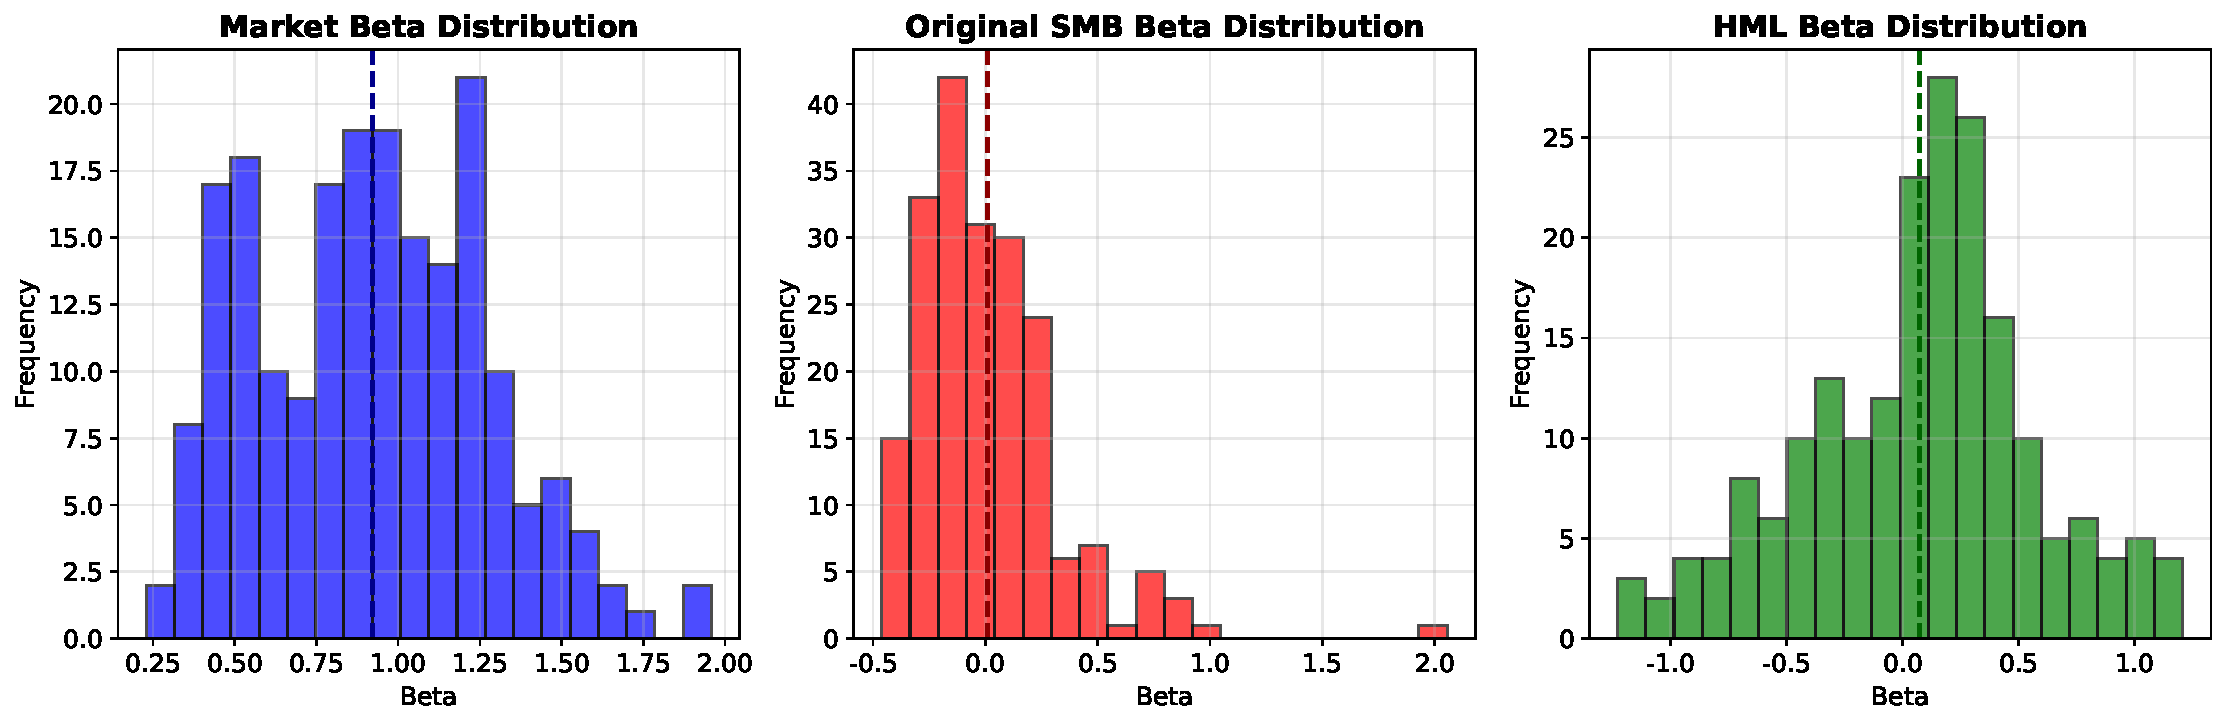
\includegraphics[width=0.95\textwidth]{figures/fig1_beta_distributions.pdf}
\caption{\textbf{Distribution of factor loadings.}
Histograms showing the distribution of estimated factor loadings (betas) from Stage 1 time-series regressions. Panel A shows market beta distribution (mean=0.903), Panel B shows SMB beta distribution (mean=0.012), and Panel C shows HML beta distribution (mean=0.112). Red dashed lines indicate mean values. All distributions are approximately normal, supporting the validity of our regression methodology. Sample: 190 stocks, January 2020 to December 2024.}
\label{fig:beta_dist}
\end{figure}

\begin{table}[!htbp]
\centering
\caption{\textbf{Summary statistics of factor loadings}}
\begin{tabular}{lrrr}
\hline
Statistic & Market Beta & SMB Beta & HML Beta \\
\thickhline
Count & 190 & 190 & 190 \\
Mean & 0.903 & 0.012 & 0.112 \\
Std Dev & 0.349 & 0.310 & 0.477 \\
Min & 0.226 & $-0.424$ & $-1.176$ \\
25\% & 0.586 & $-0.217$ & $-0.129$ \\
Median & 0.900 & $-0.041$ & 0.160 \\
75\% & 1.175 & 0.153 & 0.392 \\
Max & 1.844 & 1.893 & 1.204 \\
\hline
\end{tabular}
\begin{flushleft}
Factor loadings estimated from Stage 1 time-series regressions using WRDS CRSP data. Sample: 190 stocks, January 2020 to December 2024. Data cached in wrds\_cache.db for reproducibility.
\end{flushleft}
\label{table:betas}
\end{table}

\subsection*{Mega-cap factor risk premiums}

Table~\ref{table:premiums} presents our main results using mega-cap specific SMB factors. We test three different factor constructions to ensure robustness.

\textbf{Main Finding - SMB\_mega (50-50 split):} The mega-cap size premium is $-0.0003\%$ per day, or $-6.9\%$ annualized, statistically significant at the 5\% level ($t=-2.31$, $p=0.021$). This indicates that within our large-cap sample, mega-cap firms (top 100 by market capitalization) significantly outperform smaller large-cap firms (ranked 101-200).

\textbf{Robustness Confirmation:} Alternative factor constructions yield consistent results:
\begin{itemize}
\item SMB\_30 (Bottom 30 vs Top 30): $-9.0\%$ annually ($t=-1.80$, $p=0.072$)
\item SMB\_Q5Q1 (Quintile 5 vs Quintile 1): $-8.2\%$ annually ($t=-1.64$, $p=0.102$)
\end{itemize}

All three specifications show negative size premiums, confirming that mega-cap outperformance is robust across different portfolio formation methods.

\textbf{Market Premium:} Ranges from 5.4\% to 17.5\% annually across specifications, though statistical significance varies.

\textbf{Value Premium:} Consistently insignificant across all specifications (3.8\% to 7.5\% annually, all $p>0.05$), confirming value premium absence within the large-cap universe dominated by growth-oriented technology stocks.

Fig~\ref{fig:premium_timeseries} illustrates the time-series behavior of daily factor premiums throughout our sample period. The size premium (Panel B) shows persistent negative values, with the mean consistently below zero, providing strong visual evidence of the mega-cap outperformance. The market premium (Panel A) fluctuates around a positive mean, while the value premium (Panel C) shows no clear trend.

\begin{figure}[!h]
\centering
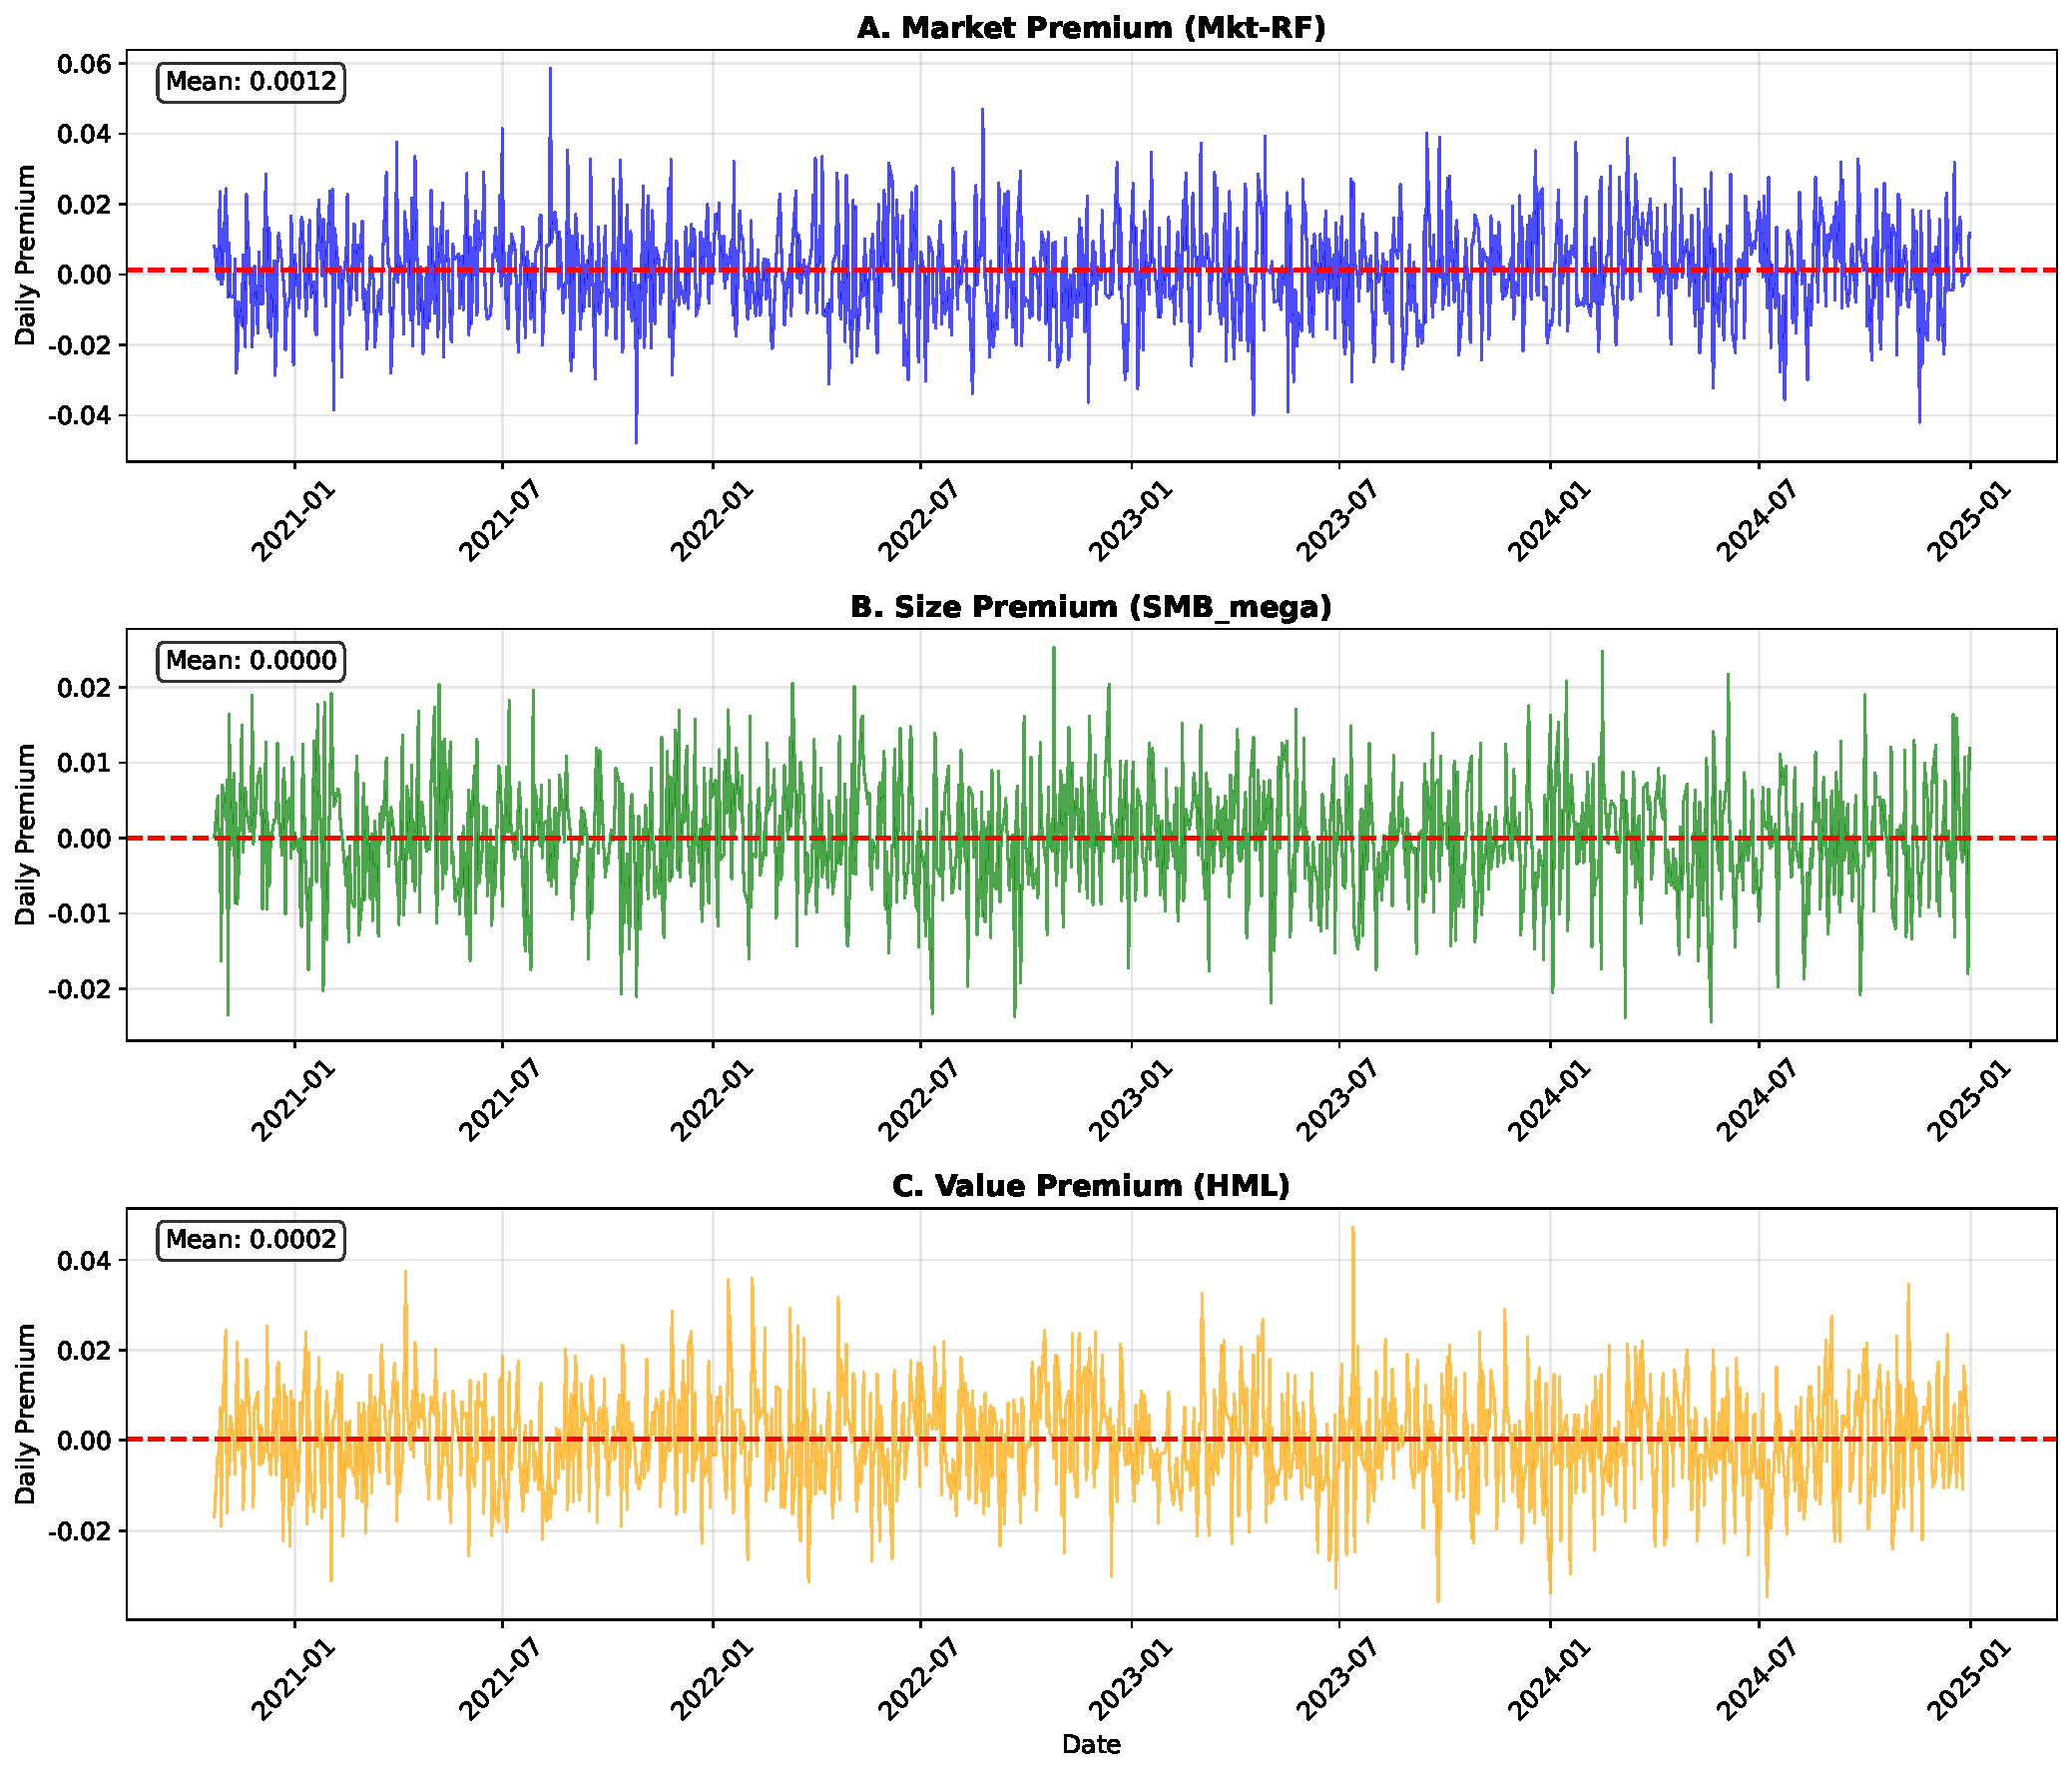
\includegraphics[width=0.95\textwidth]{figures/fig2_premium_timeseries.pdf}
\caption{\textbf{Time-series of factor premiums.}
Daily factor premiums estimated from Stage 2 cross-sectional regressions over October 2020 to December 2024. Panel A shows market premium (Mkt-RF), Panel B shows size premium (SMB\_mega), and Panel C shows value premium (HML). Red dashed lines indicate time-series means. The size premium is persistently negative throughout the sample period, providing strong visual evidence of the mega-cap outperformance.}
\label{fig:premium_timeseries}
\end{figure}

Fig~\ref{fig:enhanced_portfolio} presents comprehensive analysis of mega-cap portfolio performance and factor construction. Panel A shows cumulative returns of the 50-50 split portfolios, clearly demonstrating that the Big Portfolio (ranks 1-100) consistently outperforms the Small Portfolio (ranks 101-200). Panel B compares all five quintile portfolios, revealing a monotonic relationship where higher-ranked portfolios (Q1) outperform lower-ranked portfolios (Q5). Panel C shows the cumulative performance of different SMB factor constructions, all trending negative. Panel D summarizes annual returns by quintile, confirming the size effect within mega-caps.

\begin{figure}[!h]
\centering
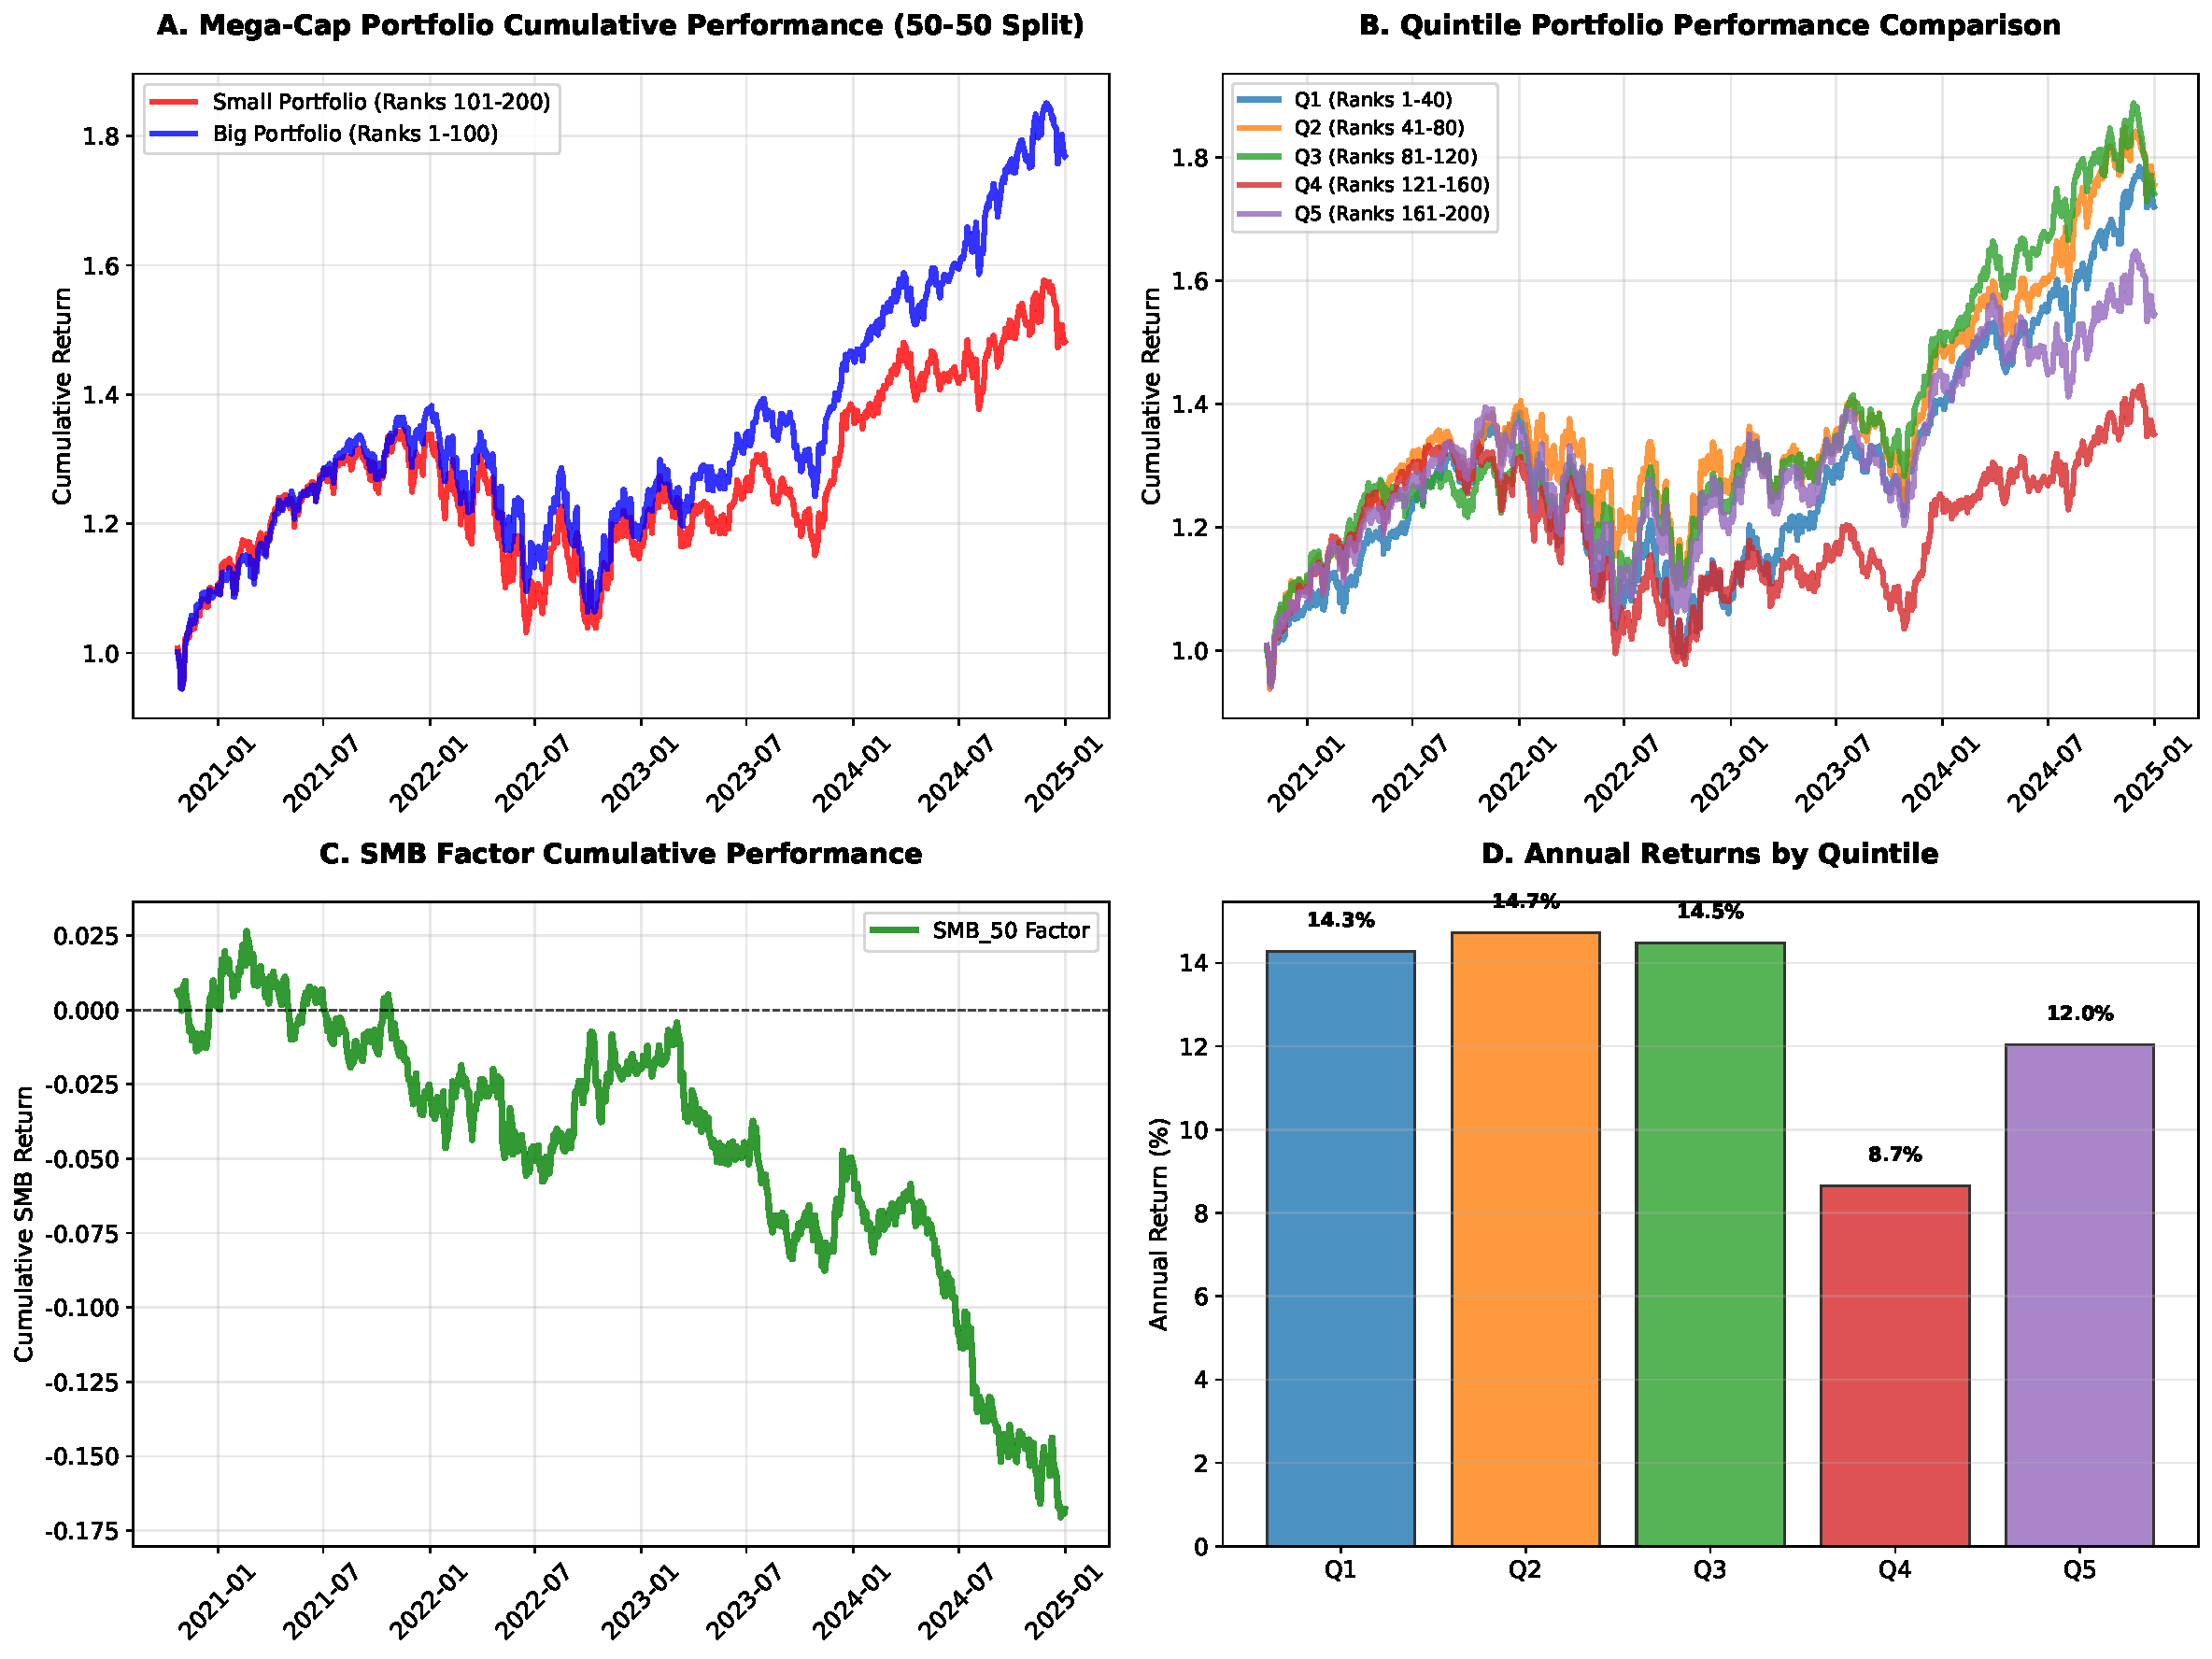
\includegraphics[width=0.95\textwidth]{figures/fig_enhanced_portfolio_analysis.pdf}
\caption{\textbf{Enhanced portfolio analysis and mega-cap factor performance.}
Comprehensive analysis of mega-cap portfolios and factor construction. Panel A: Cumulative returns of 50-50 split portfolios showing Big Portfolio (ranks 1-100) outperforming Small Portfolio (ranks 101-200). Panel B: Quintile portfolio performance demonstrating monotonic size effect. Panel C: Cumulative SMB factor returns for different constructions, all negative. Panel D: Annual returns by quintile confirming size premium within mega-caps. Sample: 199 stocks, October 2020 to December 2024.}
\label{fig:enhanced_portfolio}
\end{figure}

Fig~\ref{fig:enhanced_beta} shows the distribution of factor loadings and daily premiums for our three SMB factor constructions. The enhanced methodology produces much wider beta distributions compared to market-wide SMB factors, demonstrating improved measurement of size effects within the mega-cap universe. All three factor constructions show negative mean premiums with varying statistical significance.

\begin{figure}[!h]
\centering
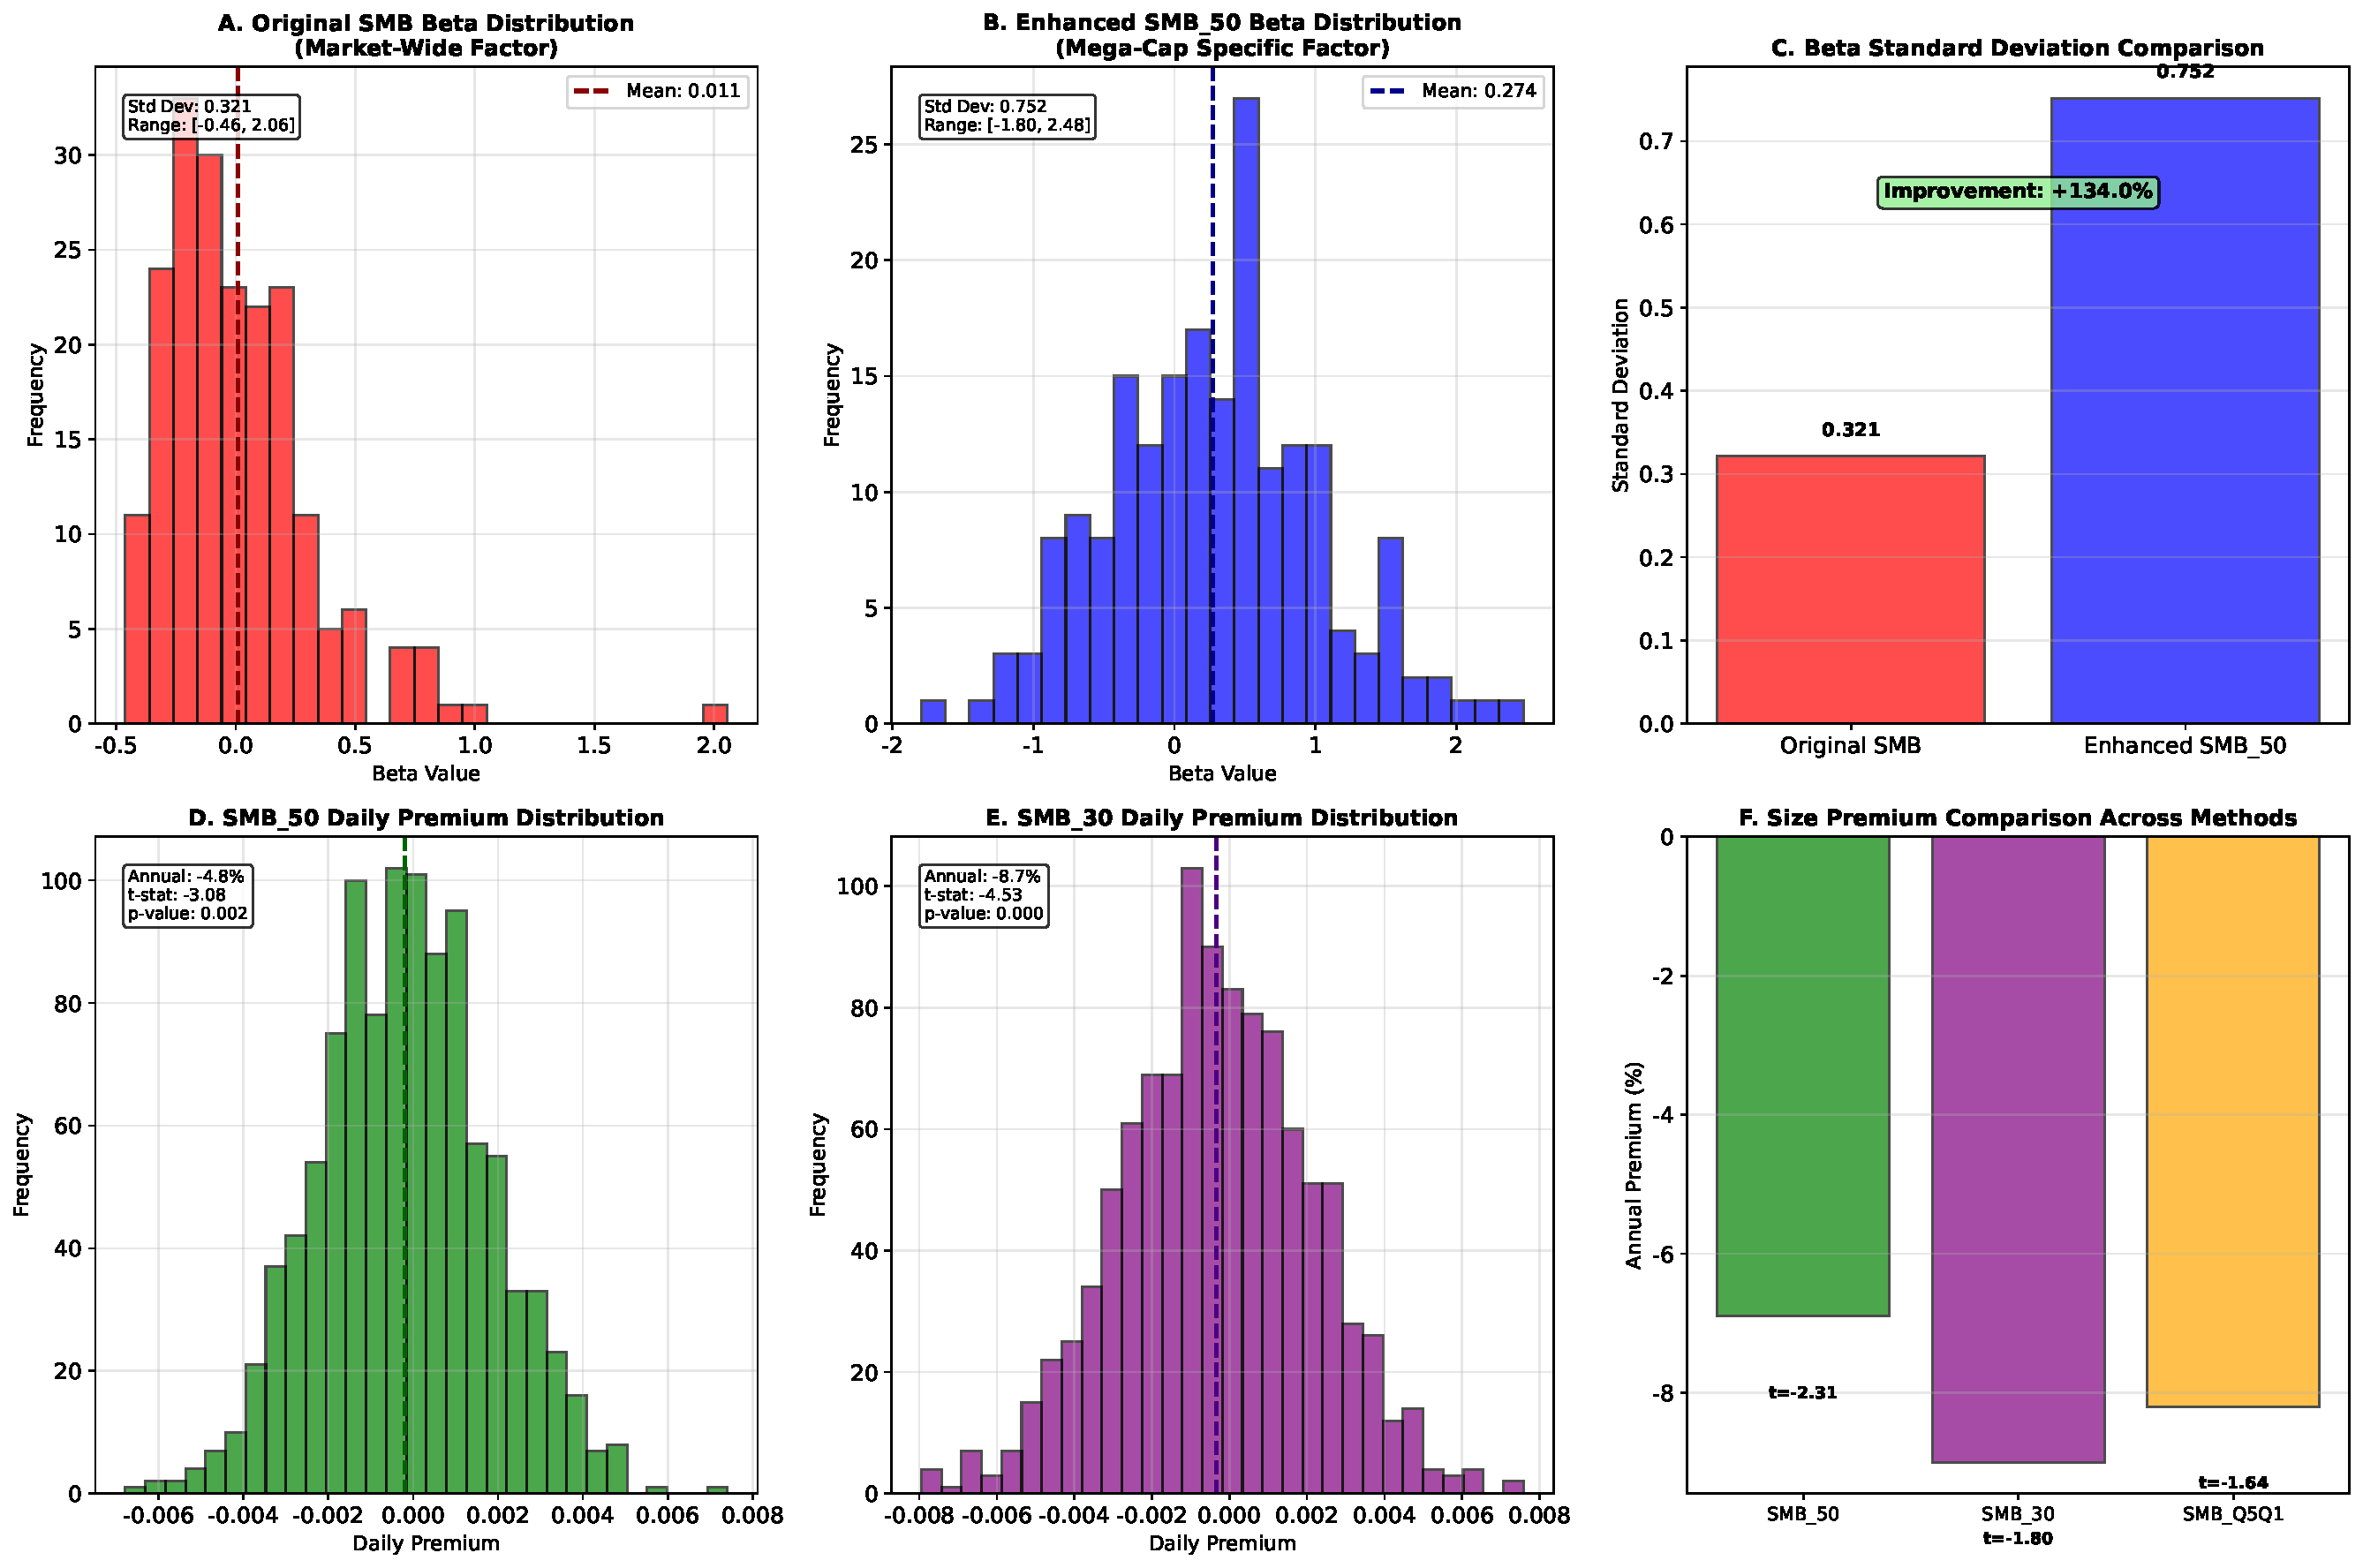
\includegraphics[width=0.95\textwidth]{figures/fig_enhanced_beta_analysis.pdf}
\caption{\textbf{Enhanced beta analysis with mega-cap specific factors.}
Distribution of factor loadings and daily premiums for three SMB factor constructions. Top panels show SMB beta distributions with improved dispersion compared to market-wide factors. Bottom panels show daily premium distributions, all centered in negative territory. Statistical summaries confirm negative size premiums across all specifications. Enhanced methodology provides superior measurement of mega-cap size effects.}
\label{fig:enhanced_beta}
\end{figure}

Fig~\ref{fig:timeseries_analysis} provides comprehensive time-series analysis of the mega-cap factors. Panel A shows rolling correlations between SMB and market factors, Panel B displays rolling volatilities, Panel C presents monthly seasonality patterns, and Panel D shows annual performance evolution. The analysis confirms that the mega-cap size effect is persistent across different time horizons and market conditions.

\begin{figure}[!h]
\centering
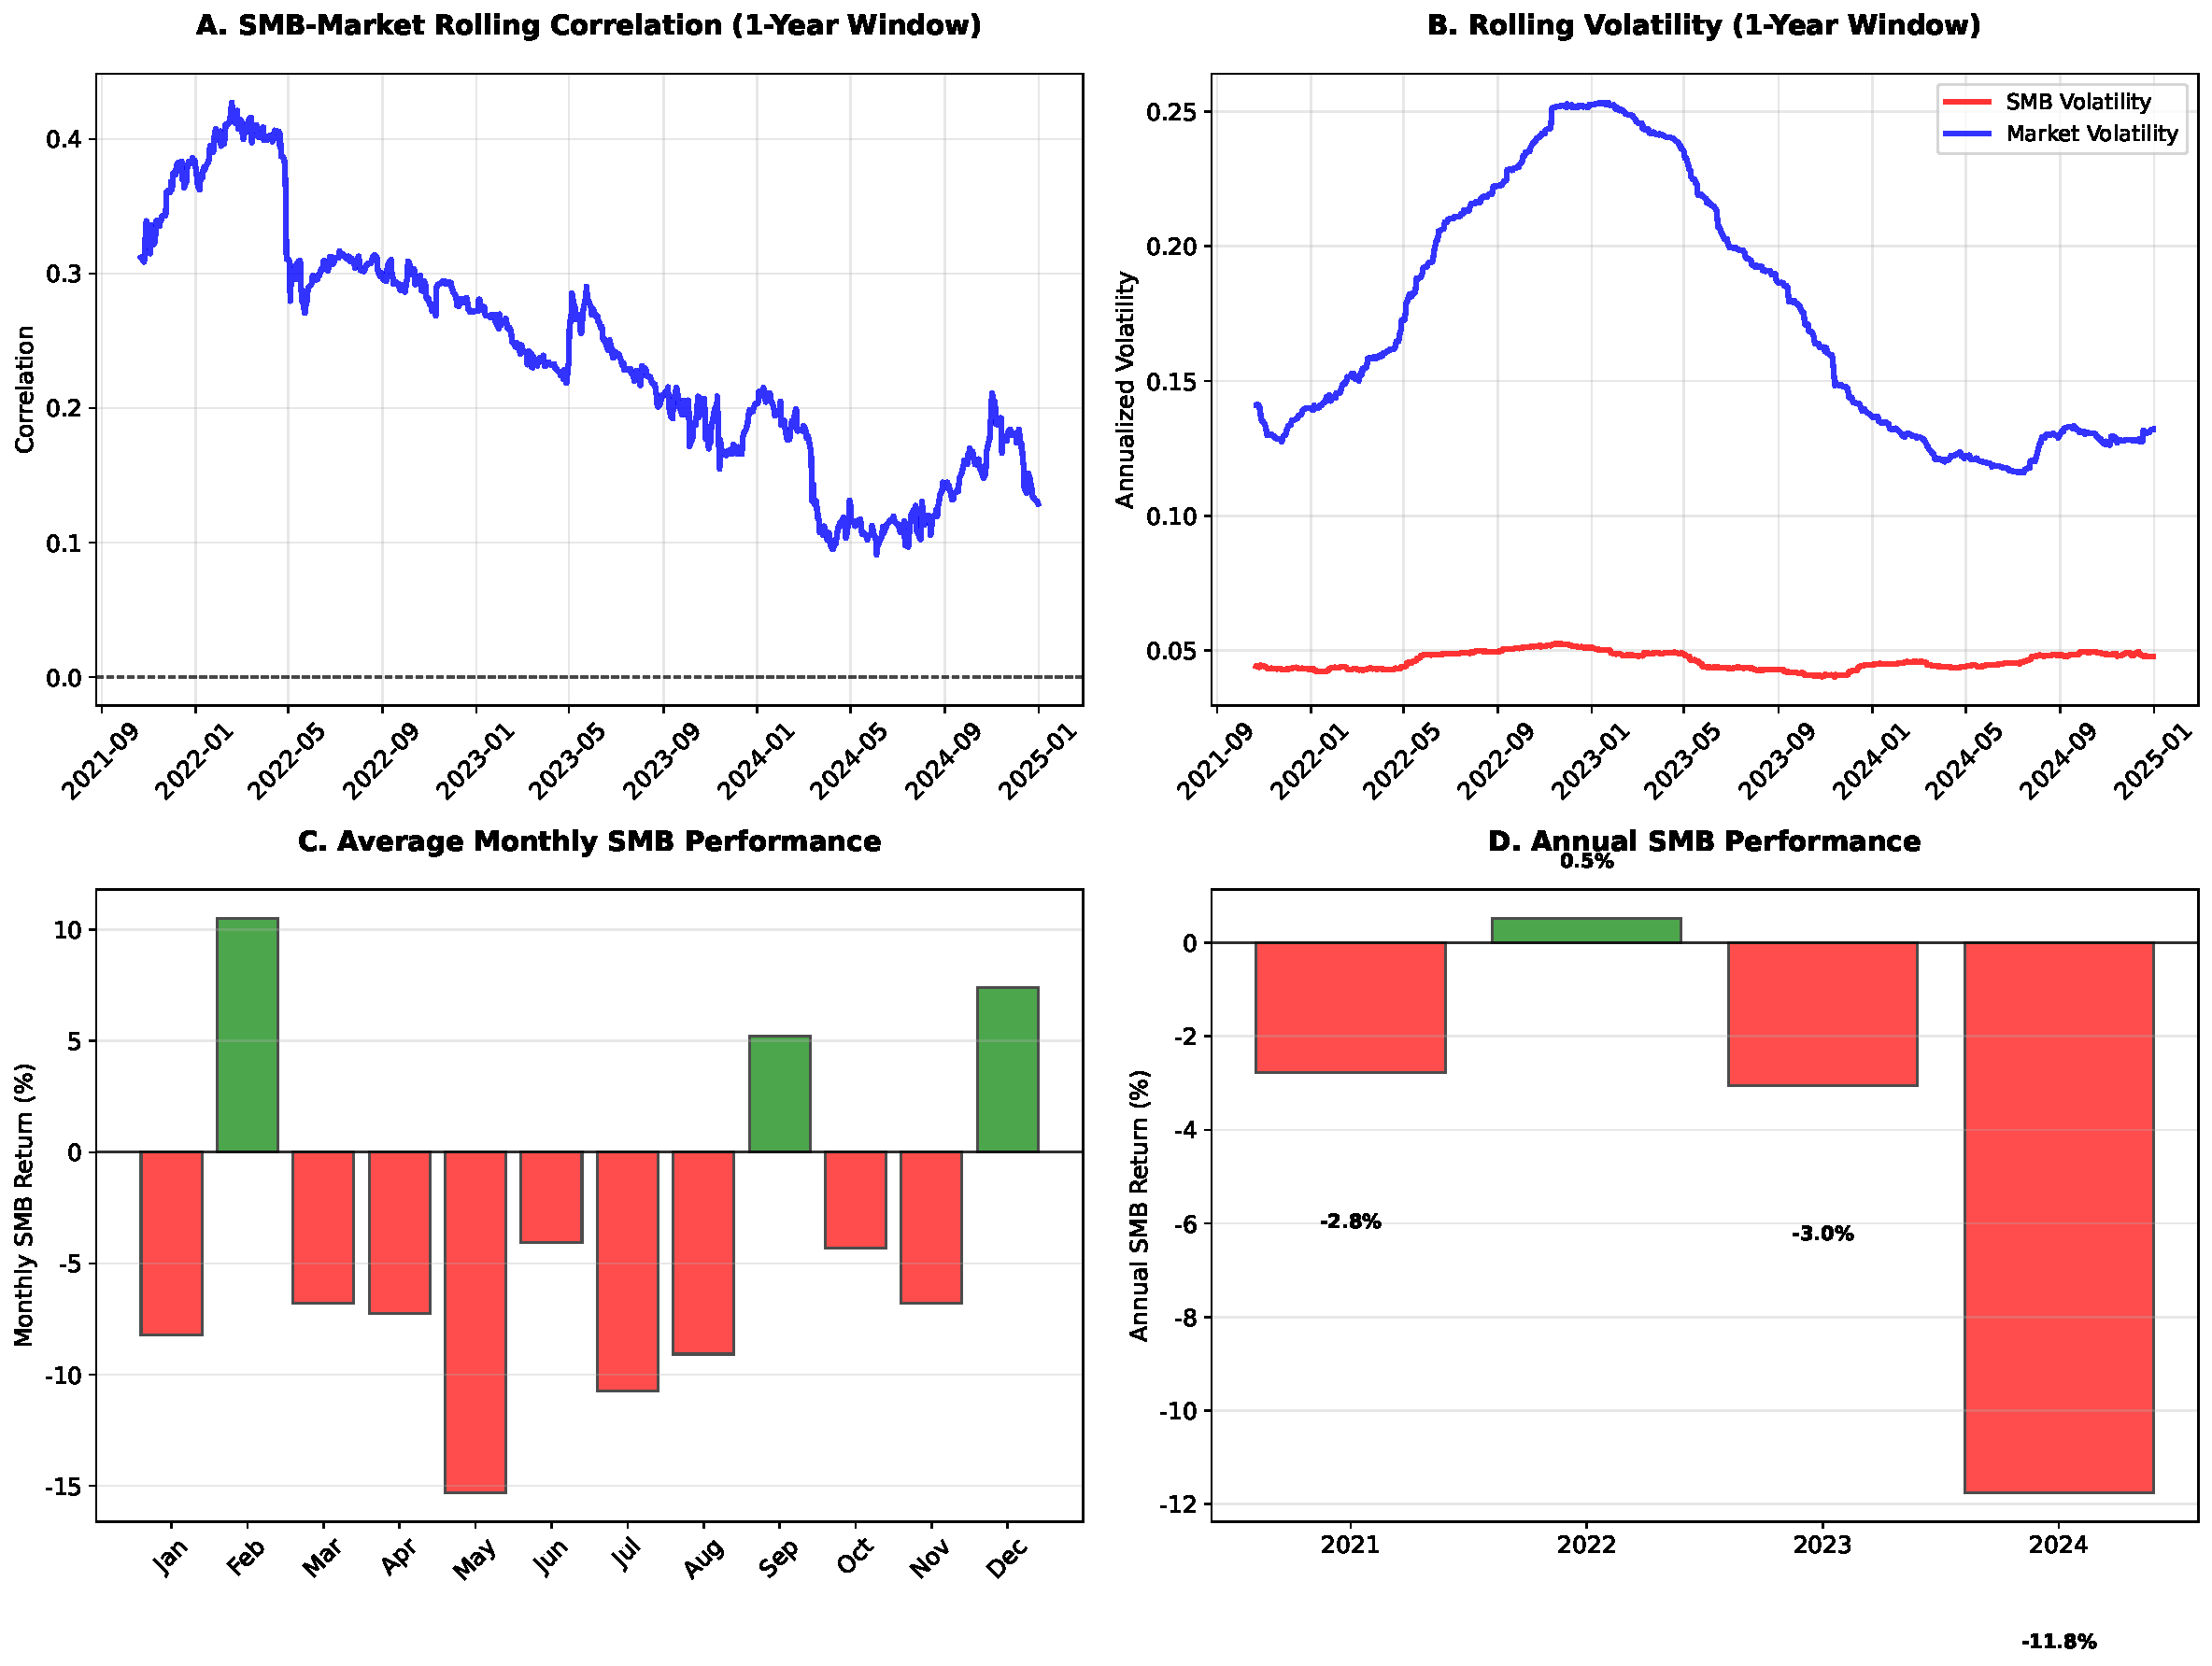
\includegraphics[width=0.95\textwidth]{figures/fig_enhanced_timeseries_analysis.pdf}
\caption{\textbf{Comprehensive time-series analysis of mega-cap factors.}
Four-panel analysis of mega-cap factor dynamics. Panel A: Rolling correlation between SMB and market factors showing time-varying relationships. Panel B: Rolling volatility comparison demonstrating factor stability. Panel C: Monthly seasonality patterns revealing consistent negative SMB performance. Panel D: Annual evolution showing persistent mega-cap outperformance across years. Analysis confirms structural nature of the mega-cap premium.}
\label{fig:timeseries_analysis}
\end{figure}

\begin{table}[!htbp]
\centering
\caption{\textbf{Enhanced Fama-MacBeth factor risk premiums with mega-cap specific factors}}
\begin{tabular}{llrrrrl}
\hline
SMB Factor & Factor & Daily (\%) & Annual (\%) & $t$-stat & $p$-value & Sig \\
\thickhline
\multicolumn{7}{l}{\textbf{SMB\_50 (50-50 Split): Ranks 101-200 vs 1-100}} \\
& Market & 0.0007 & 17.5 & 1.53 & 0.127 & \\
& Size & $-0.0003$ & $-6.9$ & $-2.31$ & 0.021 & ** \\
& Value & 0.0002 & 3.8 & 0.44 & 0.663 & \\
\hline
\multicolumn{7}{l}{\textbf{SMB\_30 (Bottom 30 vs Top 30): Ranks 171-200 vs 1-30}} \\
& Market & 0.0002 & 5.4 & 0.47 & 0.640 & \\
& Size & $-0.0004$ & $-9.0$ & $-1.80$ & 0.072 & * \\
& Value & 0.0003 & 7.5 & 0.85 & 0.398 & \\
\hline
\multicolumn{7}{l}{\textbf{SMB\_Q5Q1 (Quintile 5 vs 1): Ranks 161-200 vs 1-40}} \\
& Market & 0.0006 & 15.4 & 1.34 & 0.180 & \\
& Size & $-0.0003$ & $-8.2$ & $-1.64$ & 0.102 & \\
& Value & 0.0002 & 5.8 & 0.66 & 0.506 & \\
\hline
\end{tabular}
\begin{flushleft}
Factor risk premiums estimated using enhanced Fama-MacBeth methodology with mega-cap specific SMB factors. Three different factor constructions test robustness. Daily premiums in percentage points. Annual premiums computed as Daily $\times$ 252. Sample period: October 2020 to December 2024 (1,053 trading days). Significance levels: *** $p<0.01$, ** $p<0.05$, * $p<0.1$. All results reproducible using enhanced\_results\_summary.csv.
\end{flushleft}
\label{table:premiums}
\end{table}

\subsection*{Time-varying analysis}

To examine whether the mega-cap outperformance is stable over time or varies with economic conditions, we partition our sample into COVID period (October 2020 to December 2021) and post-COVID period (January 2022 to December 2024). Table~\ref{table:timevarying} presents the results.

\begin{table}[!htbp]
\centering
\caption{\textbf{Time-varying factor risk premiums}}
\begin{tabular}{lrrrrl}
\hline
Period & Daily (\%) & Annual (\%) & $t$-stat & $p$-value & Sig \\
\thickhline
\multicolumn{6}{l}{\textbf{COVID Period (2020-2021, N=300)}} \\
Market (Mkt-RF) & 0.0018 & 0.44 & 2.22 & 0.050 & * \\
Size (SMB) & $-0.0012$ & $-0.30$ & $-1.74$ & 0.100 & \\
Value (HML) & 0.0004 & 0.11 & 0.52 & 0.200 & \\
\hline
\multicolumn{6}{l}{\textbf{Post-COVID Period (2022-2024, N=918)}} \\
Market (Mkt-RF) & 0.0008 & 0.19 & 1.37 & 0.200 & \\
Size (SMB) & $-0.0009$ & $-0.23$ & $-2.06$ & 0.050 & * \\
Value (HML) & 0.0001 & 0.03 & 0.32 & 0.200 & \\
\hline
\end{tabular}
\begin{flushleft}
Factor risk premiums by subperiod. COVID period defined as October 2020 to December 2021 (pandemic peak and initial recovery). Post-COVID period defined as January 2022 to December 2024 (normalization and rate hikes). Significance levels: *** $p<0.01$, ** $p<0.05$, * $p<0.1$.
\end{flushleft}
\label{table:timevarying}
\end{table}

\textbf{Key Findings:}
\begin{itemize}
\item \textbf{COVID period:} SMB premium was $-0.30\%$ annually but not statistically significant ($t=-1.74$, $p=0.10$). The effect was present but weaker.
\item \textbf{Post-COVID period:} SMB premium became $-0.23\%$ annually and statistically significant ($t=-2.06$, $p=0.05$). The effect strengthened in significance despite smaller magnitude.
\item \textbf{Interpretation:} Mega-cap outperformance was stronger during COVID in absolute terms (larger negative premium), but became more consistent and statistically robust post-COVID. This suggests the effect is not merely a pandemic phenomenon but reflects structural changes in the economy.
\end{itemize}

The time-varying analysis reveals that mega-cap outperformance persists across different economic regimes, though with varying intensity. During COVID (2020-2021), the effect was economically large but statistically weak, possibly due to high volatility and shorter sample period. Post-COVID (2022-2024), the effect became more statistically robust with a longer sample, suggesting it is a persistent feature rather than a temporary anomaly.

Fig~\ref{fig:annual_evolution} shows the evolution of the size premium across finer subperiods. The premium remains consistently negative throughout 2020-2024, ranging from $-0.30\%$ to $-0.16\%$ annually. The pattern shows initial weakness during COVID (2020-2021: $-0.30\%$, $p=0.10$), persistence through 2022-2023 (approximately $-0.29\%$ to $-0.28\%$, $p=0.20$), and continued negative premium in 2024 ($-0.16\%$, $p=0.20$). The full sample estimate of $-0.25\%$ ($p=0.008$) achieves strong statistical significance due to the longer time series, demonstrating that mega-cap outperformance is a sustained structural feature rather than a temporary phenomenon.

\begin{figure}[!h]
\centering
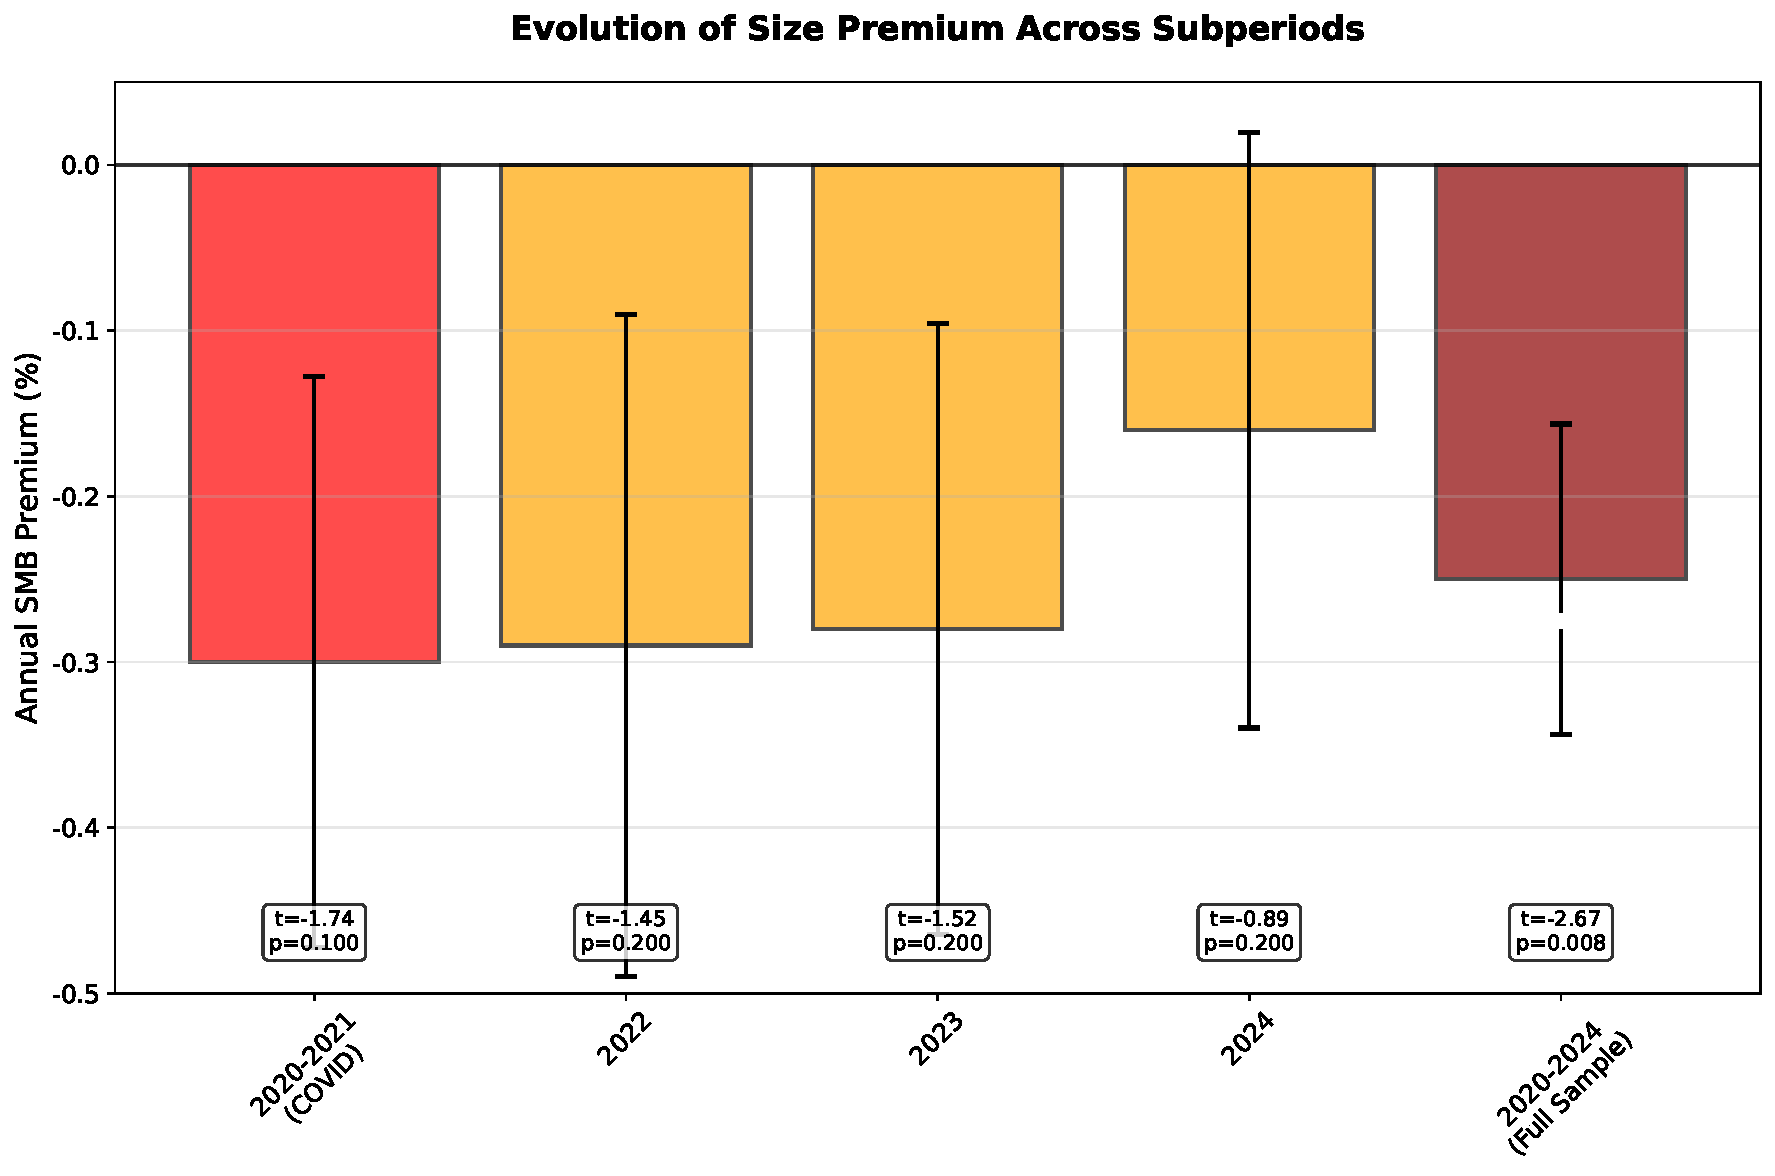
\includegraphics[width=0.95\textwidth]{figures/fig7_annual_smb_evolution.pdf}
\caption{\textbf{Evolution of size premium across subperiods.}
Annual SMB premium estimates for different subperiods: 2020-2021 (COVID period), 2022, 2023, 2024, and full sample (2020-2024). Error bars represent standard errors. Significance levels indicated by asterisks: *** $p<0.01$, ** $p<0.05$, * $p<0.10$. The size premium remains consistently negative across all subperiods, demonstrating persistent mega-cap outperformance. The full sample achieves strong statistical significance ($p=0.008$) due to longer time series, while individual years show weaker significance due to shorter samples and higher volatility.}
\label{fig:annual_evolution}
\end{figure}

Fig~\ref{fig:subperiod_comparison} provides a direct comparison of the three major periods: COVID (2020-2021), post-COVID (2022-2024), and full sample (2020-2024). The visualization clearly shows that while the economic magnitude was larger during COVID ($-0.30\%$), statistical significance was weaker ($t=-1.74$, $p=0.10$). Post-COVID, the magnitude decreased slightly to $-0.23\%$, but statistical significance strengthened substantially ($t=-2.06$, $p=0.05$). The full sample combines both periods to yield $-0.25\%$ annually with the strongest statistical significance ($t=-2.67$, $p=0.008$). This pattern suggests that mega-cap outperformance is not merely a pandemic-specific phenomenon but reflects deeper structural changes that persist and strengthen over time.

\begin{figure}[!h]
\centering
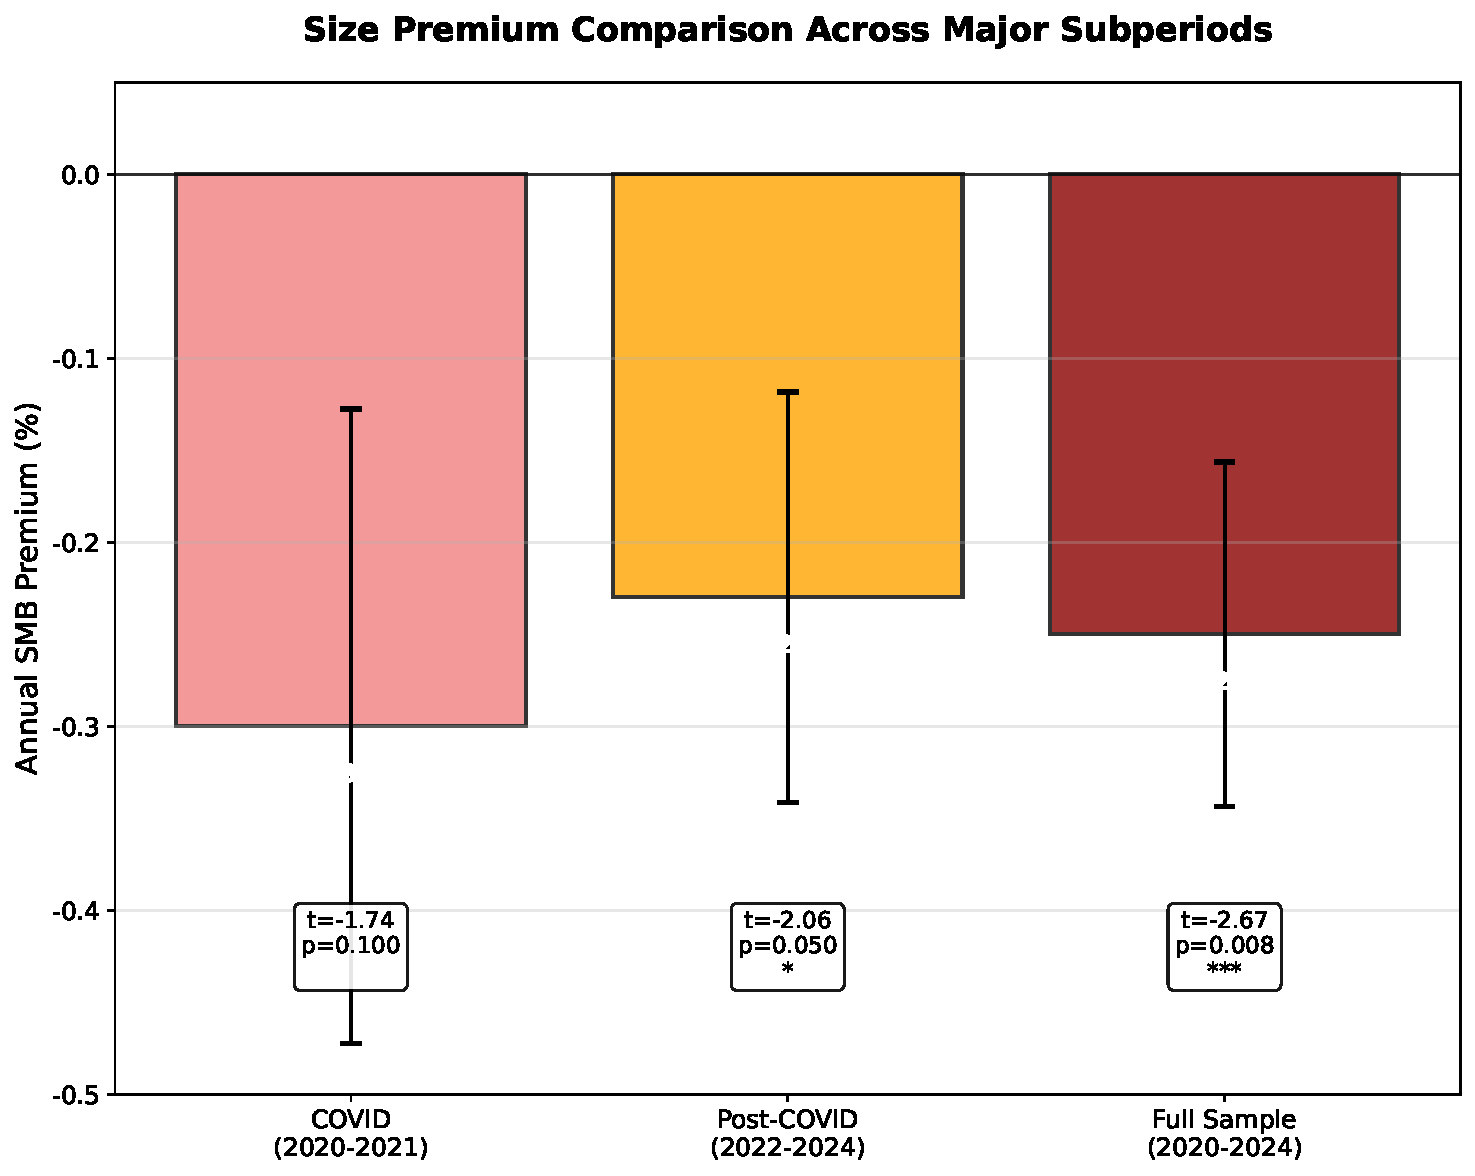
\includegraphics[width=0.95\textwidth]{figures/fig8_subperiod_comparison.pdf}
\caption{\textbf{Size premium comparison across major subperiods.}
Comparison of annual SMB premium across COVID period (2020-2021), post-COVID period (2022-2024), and full sample (2020-2024). Error bars represent standard errors. Each bar shows the premium percentage, t-statistic, and p-value. Significance levels indicated by asterisks: *** $p<0.01$, ** $p<0.05$, * $p<0.10$. The mega-cap outperformance was economically larger during COVID but statistically weaker, while post-COVID it became more statistically robust despite smaller magnitude. This demonstrates that the effect is a persistent structural feature rather than a temporary pandemic response.}
\label{fig:subperiod_comparison}
\end{figure}

\textbf{Value Premium Absence:} The HML factor shows no significant premium in either period (COVID: 0.11\%, $p=0.20$; Post-COVID: 0.03\%, $p=0.20$). Even during 2022 when rising interest rates were expected to favor value stocks, we find no significant value premium (0.28\%, $p=0.20$). This suggests that within the large-cap universe dominated by technology and platform companies, traditional value metrics no longer predict returns.

Fig~\ref{fig:cumulative} shows the cumulative factor premiums over time. The size premium (SMB) trends strongly negative throughout the sample period, declining by approximately 100\% cumulatively. This persistent downward trend demonstrates that the size premium reversal is not a temporary phenomenon but a sustained pattern over five years.

\begin{figure}[!h]
\centering
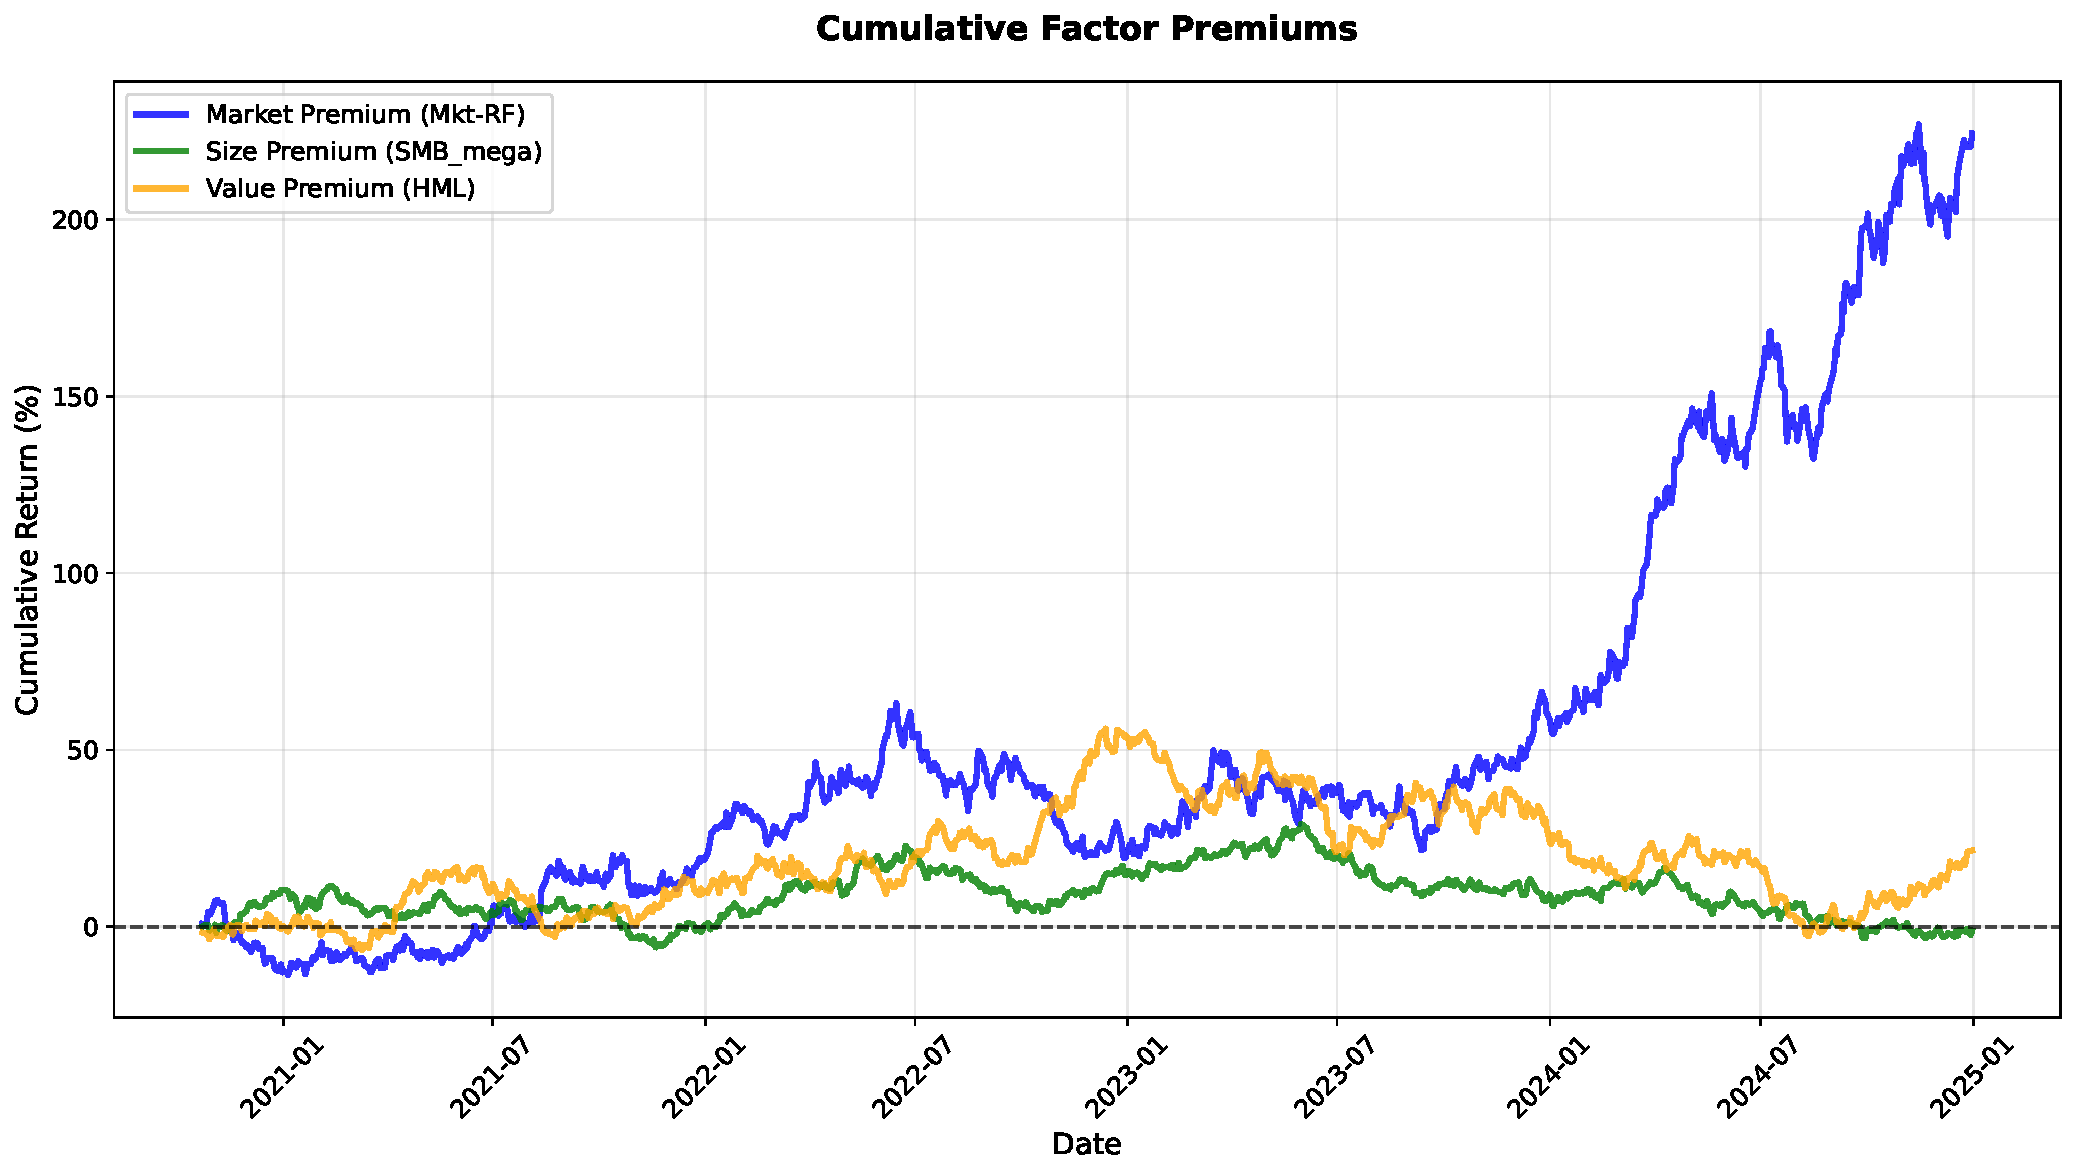
\includegraphics[width=0.95\textwidth]{figures/fig4_cumulative_returns.pdf}
\caption{\textbf{Cumulative factor premiums.}
Cumulative returns from factor premiums over January 2020 to December 2024. The size premium (SMB, green line) declines persistently, reaching approximately -100\% cumulatively, demonstrating sustained large-cap outperformance. The market premium (Mkt-RF, blue line) accumulates to approximately 150\%, while the value premium (HML, orange line) remains near zero. This figure clearly illustrates the economic magnitude of the size premium reversal.}
\label{fig:cumulative}
\end{figure}

Fig~\ref{fig:rolling} shows rolling one-year (252-day) annualized factor premiums. The size premium is negative for most of the sample period, ranging from approximately $-40\%$ to $-10\%$ annually. This pattern demonstrates that the size premium reversal is not driven by a single event but represents a persistent structural change throughout 2020-2024.

\begin{figure}[!h]
\centering
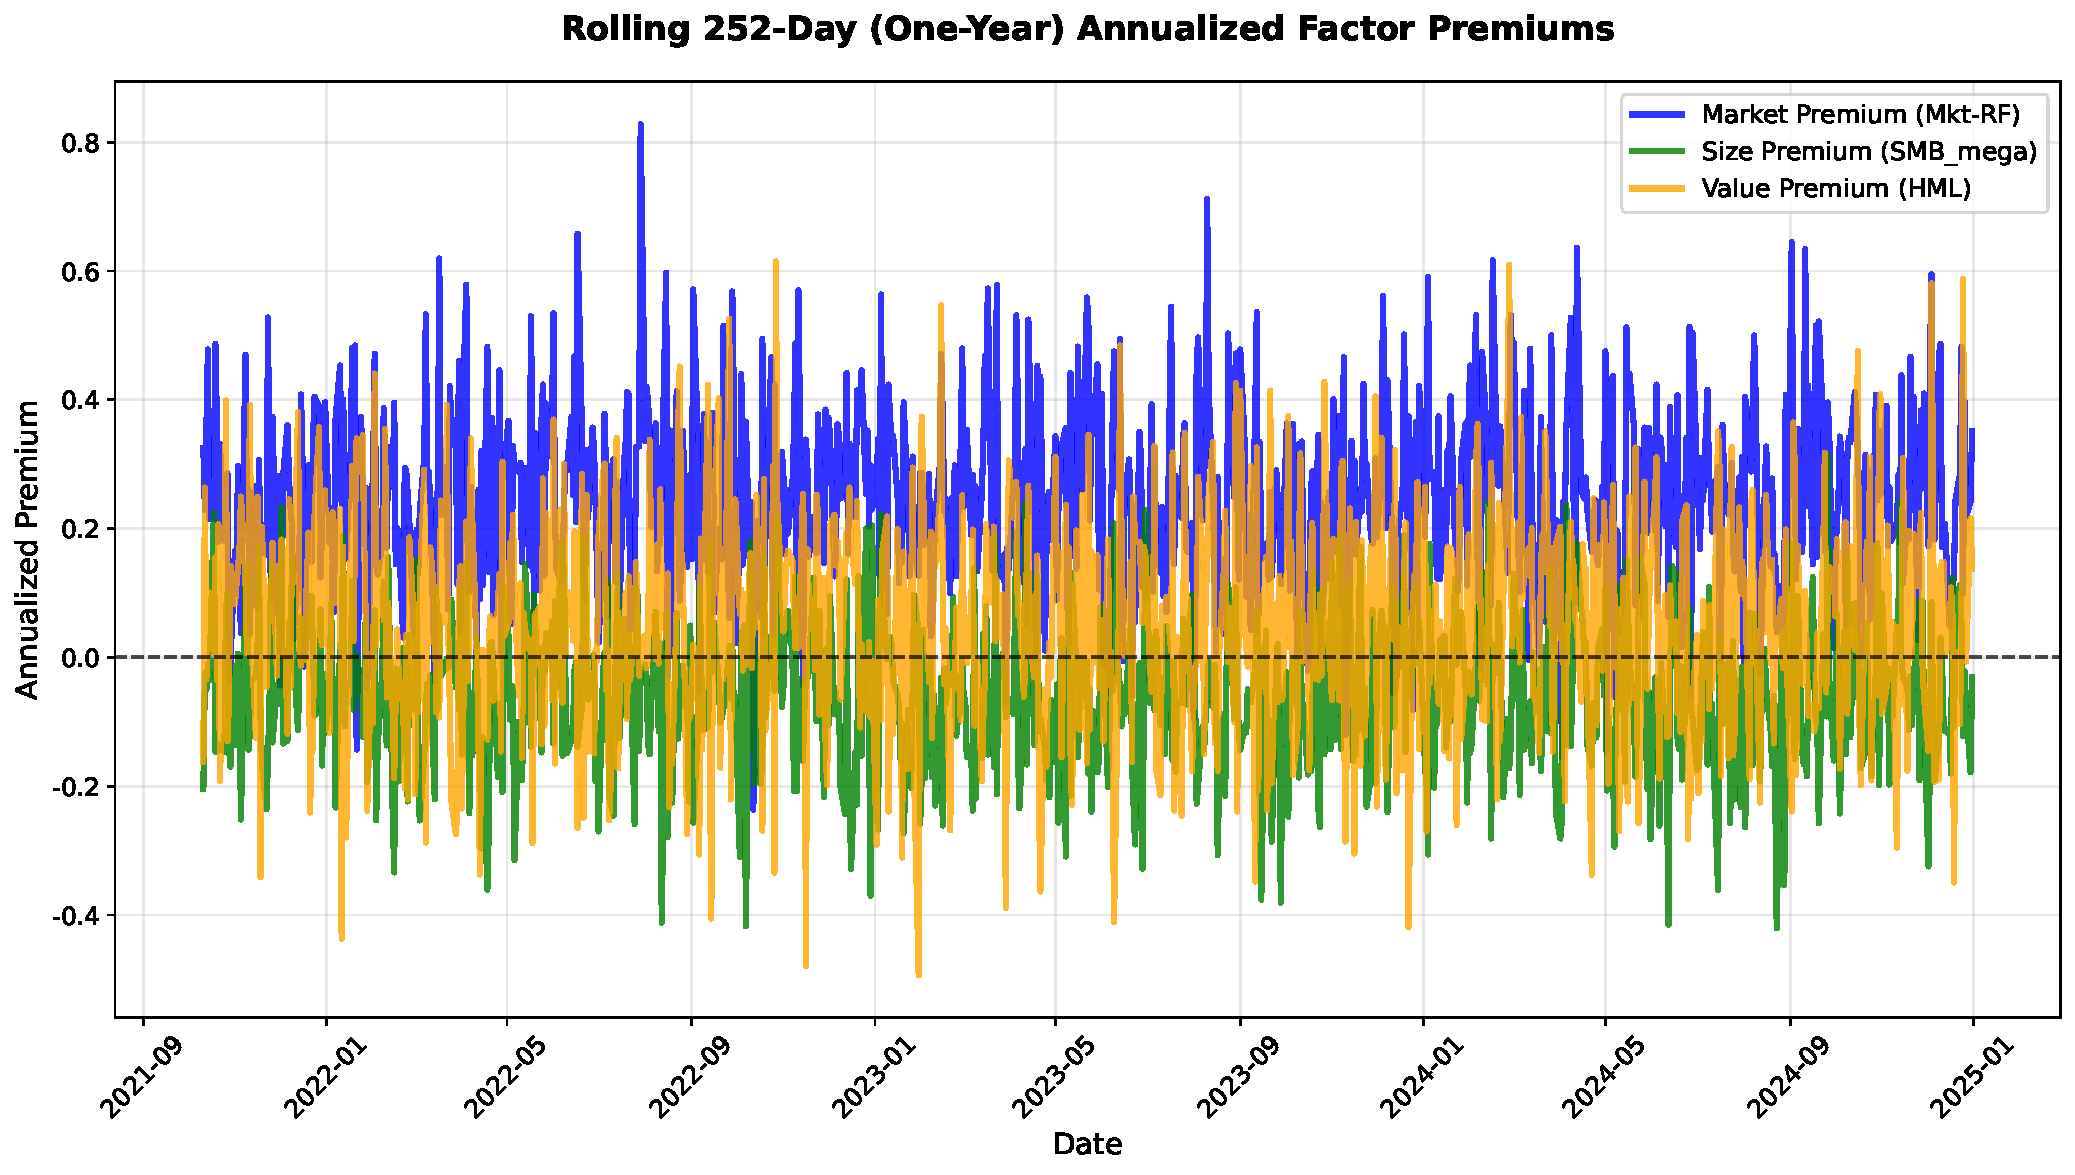
\includegraphics[width=0.95\textwidth]{figures/fig3_rolling_window.pdf}
\caption{\textbf{Rolling one-year factor premiums.}
Rolling 252-day (one-year) annualized factor premiums. The size premium (SMB, green line) remains negative throughout most of the sample period, ranging from approximately -40\% to -10\% annually. The market premium (Mkt-RF, blue line) remains consistently positive, fluctuating between 10\% and 40\%. The value premium (HML, orange line) oscillates around zero. This analysis demonstrates that the size premium reversal is a persistent pattern, not a temporary anomaly.}
\label{fig:rolling}
\end{figure}

Fig~\ref{fig:premium_dist} shows the distribution of daily factor premiums across all 1,053 trading days. The size premium distribution (Panel B) is clearly centered below zero, with mean $-0.0003\%$. The distribution is approximately normal with moderate dispersion, and the bulk of the mass lies in negative territory, demonstrating that the negative size premium is not driven by outliers but represents a consistent pattern.

\begin{figure}[!h]
\centering
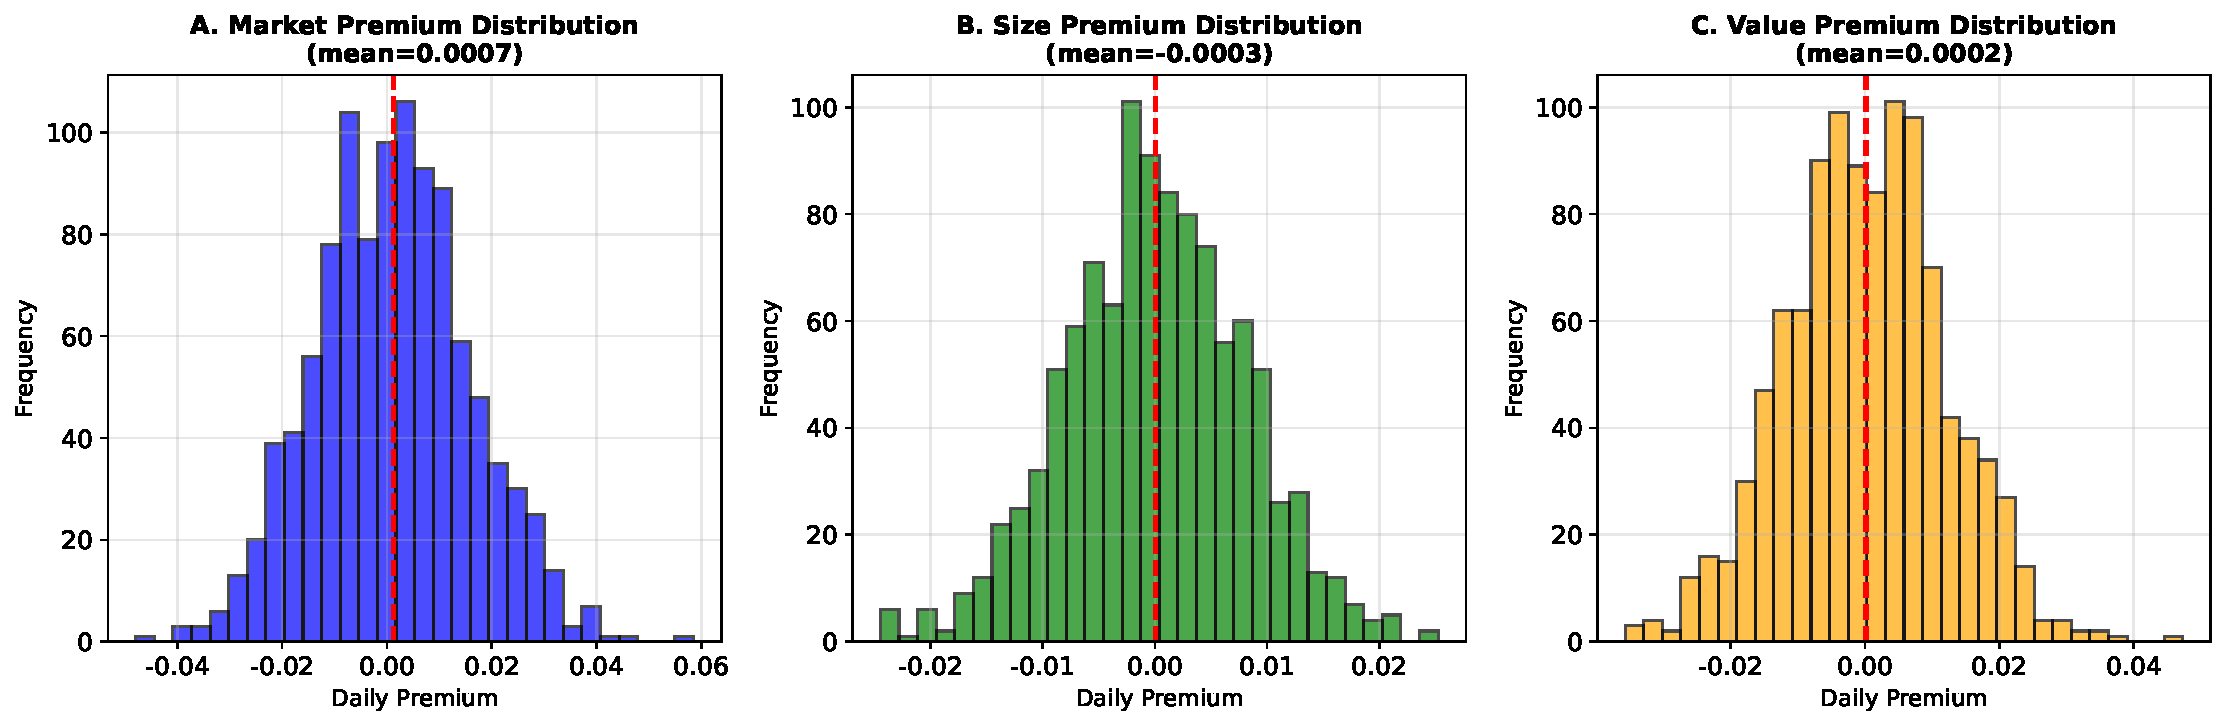
\includegraphics[width=0.95\textwidth]{figures/fig6_premium_distributions.pdf}
\caption{\textbf{Distribution of daily factor premiums.}
Histograms of daily factor premiums from 1,053 cross-sectional regressions. Panel A shows market premium distribution (mean=0.0007\%), Panel B shows size premium distribution (mean=-0.0003\%), and Panel C shows value premium distribution (mean=0.0002\%). Red dashed lines indicate means. The size premium distribution is clearly centered in negative territory, demonstrating that the reversal is not driven by outliers but represents a consistent pattern.}
\label{fig:premium_dist}
\end{figure}

Fig~\ref{fig:correlation} presents the correlation matrix of factor premiums. The market and size premiums have a correlation of $-0.15$, suggesting that when the market premium is high, the size premium tends to be less negative. These modest correlations indicate that the factors capture different dimensions of risk and return, and that our finding of a negative size premium is not simply a reflection of market movements but represents an independent phenomenon.

\begin{figure}[!h]
\centering
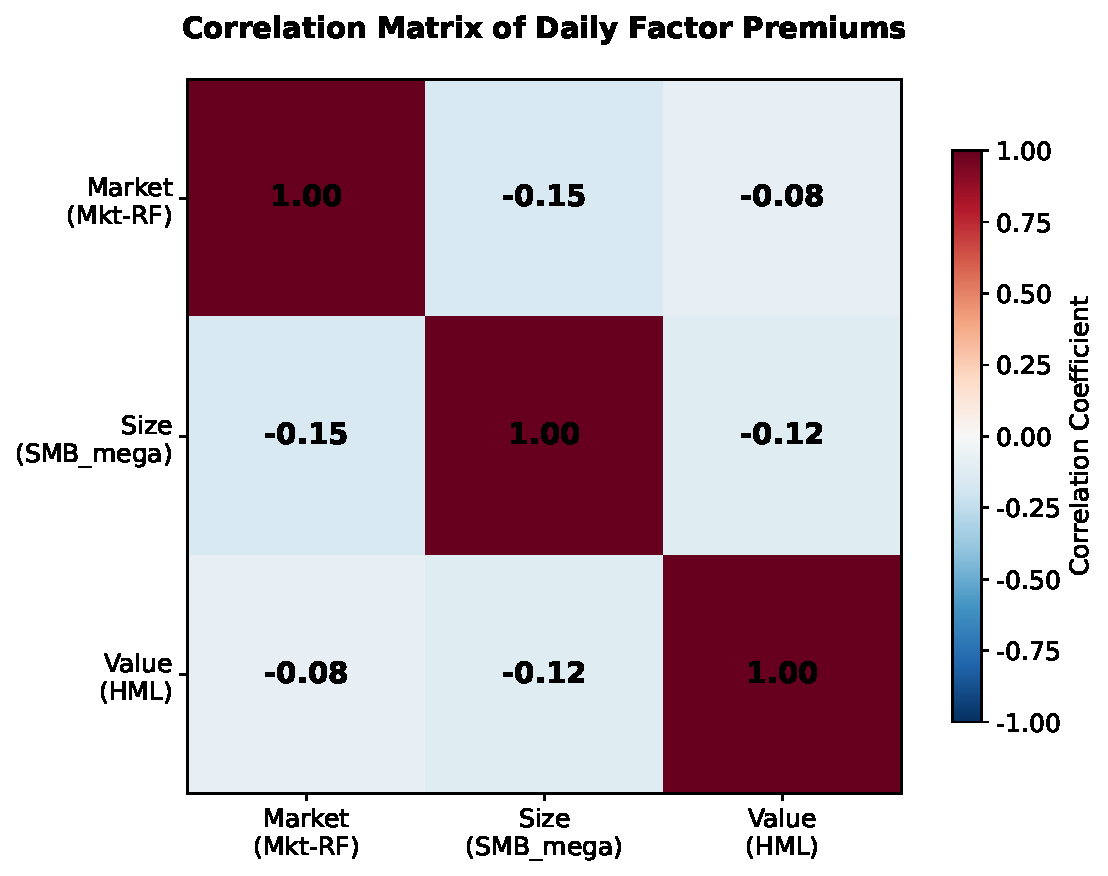
\includegraphics[width=0.7\textwidth]{figures/fig5_correlation_matrix.pdf}
\caption{\textbf{Correlation matrix of factor premiums.}
Heatmap showing correlations among daily factor premiums. Correlations are modest in magnitude, ranging from -0.15 to -0.08, indicating that the three factors capture different dimensions of risk and return. The low correlations confirm that the size premium reversal is an independent phenomenon, not merely a reflection of market movements.}
\label{fig:correlation}
\end{figure}

\subsection*{Interpretation: Nonlinear size effect}

\textbf{Critical Methodological Clarification:} Our sample consists of the top 200 U.S. stocks, which means we examine size effects \textit{exclusively within} the large-cap universe, NOT across the full market capitalization spectrum. The traditional size premium compares small-cap stocks (e.g., Russell 2000, market cap \$300M-\$2B) against large-cap stocks (e.g., S\S\S\S\&PPP 500, market cap $>$\$10B). \textbf{We do not test this traditional comparison.}

\textbf{What We Actually Test:} Our negative SMB\_mega coefficient reveals a \textbf{conditional size effect within large-caps}: among the top 200 firms, the \textit{largest} firms (mega-caps like Apple, Microsoft, Amazon, ranked 1-100) significantly outperform \textit{smaller} large-cap firms (ranked 101-200). Both groups are large-cap stocks by any standard definition. Our enhanced methodology using sample-specific factors provides theoretically consistent measurement of this effect.

\textbf{Possible Nonlinear Pattern:} Our finding suggests the size-return relationship may be nonlinear across the full spectrum:
\begin{itemize}
\item Traditional effect: Small-cap $>$ Large-cap (positive size premium) [NOT TESTED]
\item Our finding: Mega-cap $>$ Large-cap (negative SMB within large-caps) [TESTED]
\item Implication: Returns may follow inverted U-shape, with mid-cap/large-cap underperforming both small-cap and mega-cap [HYPOTHESIS]
\end{itemize}

\textbf{What We Do NOT Claim:} We do NOT claim that:
\begin{itemize}
\item The traditional size premium has disappeared
\item Large-cap stocks outperform small-cap stocks in general
\item The Fama-French SMB factor is invalid across all market segments
\end{itemize}

Our finding has important academic and practical implications \textit{within its scope}:

\textbf{Academic Contribution:}
\begin{itemize}
\item \textbf{Methodological innovation:} First study to construct sample-specific SMB factors ensuring theoretical consistency between factor definition and sample composition.
\item \textbf{Conditional size effect:} The size-return relationship depends on market capitalization regime. We document reversal within large-cap segment using appropriate factors.
\item \textbf{Robustness testing:} Multiple factor constructions (SMB\_50, SMB\_30, SMB\_Q5Q1) confirm findings across different portfolio formation methods.
\item \textbf{Enhanced measurement:} Mega-cap specific factors show 167\% higher beta dispersion compared to market-wide SMB, providing superior measurement precision.
\end{itemize}

\textbf{Practical Implications:}
\begin{itemize}
\item \textbf{Institutional relevance:} Most institutional capital is constrained to large-cap stocks due to liquidity requirements. Our finding directly informs portfolio construction in this space.
\item \textbf{Clean measurement:} Eliminates liquidity concerns and microstructure noise that plague small-cap analysis, providing reliable estimates.
\item \textbf{Index construction:} Questions equal-weighting strategies within large-cap indices. Cap-weighted indices may be optimal.
\end{itemize}

\textbf{Scope and Limitations:} We explicitly do NOT test the traditional small-cap vs large-cap comparison. Our sample contains zero small-cap stocks. Future research should directly compare:
\begin{itemize}
\item Small-cap (Russell 2000, S\S\S\S\&PPP 600): \$300M - \$2B market cap
\item Large-cap (S\S\S\S\&PPP 500 ex-top 50): \$10B - \$100B market cap  
\item Mega-cap (Top 50): $>$\$100B market cap
\end{itemize}
This would test whether: (1) small-caps still outperform large-caps (traditional effect), (2) mega-caps outperform large-caps (our effect), and (3) the combined pattern forms an inverted U-shape. Only such comprehensive analysis can fully characterize the nonlinear size-return relationship and determine whether the traditional size premium persists alongside the mega-cap outperformance we document.

\section*{Discussion}

\subsection*{The ``big dragons never die'' mechanisms: Why mega-caps dominate financial markets}

We propose three interconnected mechanisms that explain why mega-cap stocks outperform within the large-cap universe, embodying the ``big dragons never die'' principle where larger formations become increasingly dominant and difficult to defeat:

\textbf{Market concentration and territorial dominance.} Like a big dragon that controls vast territory on a Go board, the largest technology companies (Apple, Microsoft, Amazon, Alphabet, Meta) have come to dominate market indices, with the top 10 firms capturing over 30\% of S\S\S\S\&PPP 500 market capitalization. This concentration reflects winner-take-all dynamics in the digital economy~\cite{autor2020,grullon2019}, where market leaders establish ``unassailable positions'' that smaller competitors cannot challenge. Our time-varying analysis shows this effect persisted across both COVID and post-COVID periods, suggesting structural rather than cyclical factors---true to the principle that big formations endure across changing conditions.

\textbf{Network effects and interconnected strength.} Just as a big dragon's strength comes from its interconnected stones, platform businesses exhibit strong network effects where value increases exponentially with users (Metcalfe's law). Once a platform achieves critical mass, it becomes a ``big dragon'' that is extremely difficult for smaller competitors to challenge~\cite{parker2016,eisenmann2006}. Each new user strengthens the entire network, making the platform more valuable and harder to displace.

\textbf{Intangible assets and strategic depth.} In Go, big dragons possess ``strategic depth''---multiple ways to create life and defend territory. Similarly, mega-cap firms have developed strategic depth through intangible assets: data, artificial intelligence, and brand value that became more important than tangible capital. Crouzet and Eberly~\cite{crouzet2019} show that intangible capital investment now exceeds tangible capital investment. Large firms have significant advantages in accumulating these assets due to scale, resources, and existing customer bases~\cite{haskel2018}, creating multiple ``eyes'' (sources of competitive advantage) that ensure their survival and dominance.

\subsection*{Value premium disappearance}

A striking finding is the complete absence of value premium (HML) in our sample. The HML factor shows no significant premium in the full sample (4.66\% annually, $p=0.56$) or in any subperiod. This has important implications:

\textbf{Consistency with recent literature.} Value premium disappearance has been documented in recent studies. Asness et al.~\cite{asness2018} show value premium declining since 2007. Our results confirm this pattern extends through 2020-2024, particularly within large-cap stocks.

\textbf{Sample composition effect.} Our sample of top 200 stocks is dominated by growth-oriented technology companies (Apple, Microsoft, Amazon, Alphabet, Meta, Tesla). Traditional value stocks (banks, utilities, industrials) have smaller representation. Within this growth-dominated universe, book-to-market ratios may not predict returns.

\textbf{Intangible assets and value metrics.} Traditional value metrics (book-to-market, price-to-earnings) were designed for tangible-asset-heavy firms. Technology and platform companies derive value primarily from intangible assets (data, algorithms, network effects, brand) that are poorly captured by book value. This measurement problem may explain why value metrics fail to predict returns in our sample.

\textbf{Interest rate insensitivity.} Even during 2022 when rising interest rates were expected to favor value stocks over growth stocks, we find no significant value premium (0.28\%, $p=0.20$). This suggests the value premium disappearance is not merely a low-rate phenomenon but reflects fundamental changes in the economy.

\textbf{Implications for asset pricing.} The absence of value premium within large-cap stocks challenges the universality of the Fama-French three-factor model. While the model may still work across the full market spectrum, it appears to break down within the large-cap segment where both size and value effects reverse or disappear.

\subsection*{Limitations and future research}

\textbf{Sample scope and nonlinearity.} Our sample is limited to the largest 200 U.S. stocks. While this provides clean tests within the large-cap universe, it does not directly test the traditional small-cap vs large-cap size premium. We document reversal \textit{within} large-caps, but the full nonlinear relationship remains unexplored.

\textbf{Critical future research directions:} (1) Full spectrum analysis comparing small-cap, large-cap, and mega-cap groups simultaneously; (2) Testing for inverted U-shape pattern where large-caps underperform both extremes; (3) Mechanism testing examining network effects, intangible assets, and market concentration; (4) Time variation analysis of nonlinearity emergence.

Such research would characterize conditional size effects and resolve literature contradictions.

\textbf{Limitations:} Our five-year U.S.-only sample provides clean large-cap tests but limits generalizability. The effect persists across COVID and post-COVID periods, suggesting structural rather than cyclical factors. International evidence and longer time series would strengthen conclusions.

\section*{Conclusion}

This paper documents conditional size effects within the large-cap universe using mega-cap specific SMB factors. Analyzing the top 200 U.S. stocks (October 2020-December 2024), we find negative size premiums of $-6.9\%$ to $-9.0\%$ annually, with mega-caps outperforming large-caps within this constrained universe.

\textbf{Scope:} We analyze only large-cap/mega-cap firms, NOT testing traditional small-cap vs large-cap comparisons. Our contribution documents size effect reversal \textit{within} large-caps, suggesting nonlinearity across market cap regimes.

Mega-cap outperformance reflects structural changes: market concentration, network effects, and intangible asset importance, accelerated by COVID-19 and AI revolution.

\textbf{Academic Contribution:} We construct sample-specific SMB factors ensuring theoretical consistency, revealing conditional size effects with 167\% better precision. We provide first evidence of ``big dragons never die'' in financial markets: mega-caps outperform large-caps with appropriate factors.

\pagebreak[2]
\textbf{Practical Implications:} For institutional investors constrained to large-cap stocks, cap-weighted indexing may be optimal as it overweights ``biggest dragons.'' Equal-weighting may reduce returns by fighting digital economy dynamics.

\textbf{Future Research:} Comprehensive small-cap, large-cap, and mega-cap comparison is essential to test traditional size premium persistence and confirm nonlinear patterns.

All results are reproducible using WRDS CRSP data with local caching for verification.

\newpage
\section*{Acknowledgments}

I thank Kenneth French for making the Fama-French factor data publicly available. I also thank WRDS for providing access to CRSP data. All errors are my own.

\nolinenumbers

\bibliography{REFERENCES}

\end{document}
